\documentclass[11pt]{article}

\usepackage[margin=1in]{geometry}
\usepackage{amsmath,amssymb}
\usepackage{graphicx}
\usepackage[colorlinks=true,linkcolor=blue,citecolor=blue,urlcolor=blue]{hyperref}
\usepackage{natbib}
\setlength{\emergencystretch}{2em}

\title{Delayed Collapse of a Degenerate Core at Its Maximum Mass:\\
General-Relativistic Instability and the Fold-Passage Law}

\author{Gracen Ownby}
\date{}

\begin{document}
\maketitle

\begin{abstract}
Paper~B of this series finds that no known classical matter model with an independent mass parameter sources the mass-dependent regularized core studied in Papers~A and~B (nonlinear electrodynamics does, but only with the mass tied to a magnetic charge). This paper asks the dynamical question that leaves open: what does a degenerate stellar core do as it is pushed to its maximum mass, and how long does it take? For the idealized cold electron gas we (i)~locate the maximum mass with the Tolman--Oppenheimer--Volkoff equation ($M_{\max}=1.4166\,M_\odot$, within $0.07\%$ of the Chandrasekhar--Tooper value); (ii)~implement Chandrasekhar's general-relativistic pulsation equation and tighten the fundamental eigenvalue by Rayleigh--Ritz to $\sigma^2=-28.55\ {\rm s}^{-2}$ ($e$-folding time $0.187$~s) at the test configuration, passing the exact turning-point test (the eigenvalue vanishes where the mass peaks) to within $0.007\%$ in central density for five equations of state, a test our first implementation failed and that exposed two errors we correct and document; (iii)~take the nonlinear outcome (collapse, not migration, for compressive perturbations) from the established numerical-relativity literature; (iv)~build a calibrated one-degree-of-freedom nonlinear model, compared with an independent spherical general-relativistic Lagrangian evolution, which reproduces the time to half the initial radius to $0.4\%$ (a test mainly of the shared fold coefficients) and the plunge to $1$--$3\%$; and (v)~treat a star that reaches the maximum by slow accretion as a ramped saddle-node bifurcation described by the first Painlev\'e equation, which gives a collapse delay $t=3.41\,(4a/\kappa^2\dot M)^{1/5}$ in terms of two exact-GR fold coefficients, a seed set by the ramp, a mass overshoot below $10^{-10}\,M_\odot$ (conservative case; at most $10^{-8}\,M_\odot$ with damping), a $1$--$2\%$ composition dependence ($12\%$ for a counterfactual $^{56}$Fe star), and a location unaffected by dissipation, which only lengthens the delay. The use of Painlev\'e~I at a fold of the equilibrium sequence of a self-gravitating fluid is not new (Newtonian supernova cores: Pomeau et al., Chavanis et al.); the application at the general-relativistic turning point with exact fold coefficients, and the delay law, are new as far as we found. The Lagrangian evolution reaches a first trapped shell of $0.25\,M_\odot$, but that, like every timescale here, is a property of the idealized gas, which neither neutronizes nor bounces; Paper~D replaces it by a dense-matter equation of state and finds a bounce.
\end{abstract}

\section{Introduction}
\label{sec:intro}

This series studies a Hayward-type regular black hole whose regularization scale is tied to the mass, $\varepsilon^3=2GM\ell^2/c^2$, so that the core density is independent of $M$. Paper~A \citep{PaperA} treats the exterior (evaporation toward the critical mass at which the horizons merge, and the radiation's entanglement entropy). Paper~B \citep{PaperB} asks what sources the core and finds that no classical source with an independent mass does (nonlinear electrodynamics supplies it only with the mass tied to a magnetic charge). Neither says whether a real collapsing star would approach the regime in which the question arises. This paper and Paper~D \citep{PaperD} address that, for the most natural candidate: a degenerate stellar core driven to its effective maximum mass.

That a white dwarf above an effective maximum mass is unstable is old: the relativistic degenerate-gas equation of state and its limiting mass go back to Chandrasekhar \citep{Chandrasekhar1935}, the radial $\Gamma_1=4/3$ threshold to Ritter, as discussed by Pekeris \citep{Pekeris1938}, and the general-relativistic instability of white dwarfs near the limiting mass to Chandrasekhar and Tooper \citep{ChandrasekharTooper1964}. The turning-point principle that places the onset of instability at the mass maximum goes back to Harrison, Thorne, Wakano and Wheeler \citep{HTWW1965} (Sorkin \citep{Sorkin1981} gives a general criterion for the onset of instability at a turning point) and has been proved rigorously for spherical barotropic stars, under conditions on the equation of state, by Had\v{z}i\'c and Lin \citep{HadzicLin2021}. We therefore do not claim the instability as new. What we supply is (a)~a documented, independently tested implementation of Chandrasekhar's equation with an exact external test, which is also how we found and removed two errors (Section~\ref{sec:turning-point-test}); and (b)~the quantitative dynamics that follow: the timescale of the collapse and, for accretion, the delay between crossing the maximum and the collapse (Section~\ref{sec:timescale}).

The paper is organized as follows. Section~\ref{sec:eos} gives the equation of state and equilibrium structure. Section~\ref{sec:linear} is the linear core: the Newtonian reference solver, Chandrasekhar's general-relativistic equation, Rayleigh--Ritz, the turning-point test, and the canonical-energy correspondence. Section~\ref{sec:nonlinear-outcome} takes the qualitative nonlinear outcome from the numerical-relativity literature. Section~\ref{sec:timescale} contains the nonlinear timescale model, its two-mode extension, the dependence on composition, the fold passage for accretion with its dissipation, and an inhomogeneous Lagrangian test. Section~\ref{sec:discussion} states what is and is not established. Earlier exploratory work, including a first neutronized equation of state, two nonlinear numerical attempts on it and a derivation of the Misner--Sharp equations, is in the supplementary technical report \citep{OwnbyPhase2} and is not used here, apart from the Newtonian Galerkin solver and its Pekeris validation (Section~\ref{sec:galerkin-main}), whose scripts are in the report's \texttt{ancillary/linear\_perturbation} directory.

\section{A real degenerate-matter equation of state}
\label{sec:eos}

\subsection{Chandrasekhar degeneracy and its limit}

We use the Chandrasekhar (1935) equation of state for a relativistic degenerate electron gas exactly, parametrized by $x\equiv p_F/(m_ec)$,
\begin{equation}
\rho=\mu_em_u\frac{8\pi}{3}\left(\frac{m_ec}{h}\right)^3x^3,\qquad P=\frac{\pi m_e^4c^5}{3h^3}f(x),\qquad f(x)=x(2x^2-3)\sqrt{1+x^2}+3\sinh^{-1}x,
\end{equation}
$\mu_e=2$. This reproduces the correct polytropic limits ($\Gamma=5/3$ for $x\ll1$, $\Gamma=4/3$ for $x\gg1$) to four significant figures, and a Newtonian hydrostatic sequence built from it reproduces the Chandrasekhar mass ($1.456\,M_\odot$ for $\mu_e=2$ with the constants used here) as its high-density asymptote, without ever exceeding it --- the well-known fact that pure electron degeneracy alone never produces a true maximum mass, only an asymptote.

\subsection{Why neutronization is not the limiting mechanism}
\label{sec:neutronization-main}

Electron capture softens the pressure above $\rho\sim10^{12}$--$10^{13}$~kg/m$^3$, and a simplified single-nuclide treatment (semi-empirical mass formula, $A=12$) gives a maximum mass. That first attempt was quantitatively wrong: against the precision treatment of Rotondo, Rueda, Ruffini and Xue \citep{RotondoRRX2011}, which combines the full TOV equation, self-consistent $\beta$-equilibrium and Coulomb lattice corrections, its critical density was off by a factor of $\sim9$ and its mass by $\sim12\%$ for $^{12}$C, because for $^{4}$He and $^{12}$C it is general relativity (the Chandrasekhar--Tooper effect \citep{ChandrasekharTooper1964}) and not neutronization that sets the maximum mass. The preliminary configuration and the nonlinear experiments performed on it are documented in the supplementary technical report \citep{OwnbyPhase2} and are not used here.

\subsection{The dominant mechanism is general-relativistic, not neutronization, and the corrected structure}
\label{sec:gr-corrected}

Since Rotondo et al.\ identify general relativity, not neutronization, as the mechanism that actually limits a Carbon-12 white dwarf's mass, we redo the equilibrium structure using the pure (non-neutronized) Chandrasekhar equation of state --- already validated above against the Newtonian Chandrasekhar mass --- with the TOV equation instead of Newtonian hydrostatic equilibrium, dropping neutronization. This is self-consistent at the density where the mechanism sets in for $^{4}$He and $^{12}$C, but not at the fiducial test density below for $^{12}$C, which lies above its inverse-$\beta$ threshold (Section~\ref{sec:composition}); neutronization there would soften the equation of state further, which we do not model.

We validated this directly against history before trusting it on anything new: Chandrasekhar \& Tooper \citep{ChandrasekharTooper1964} treated this exact combination (pure degenerate-electron EOS, full GR); the critical mass $M_{\rm crit}=1.4176\,M_\odot$ attributed to that paper is quoted by \citet{MathewNandy2014}, whose own relativistic integration gives $1.4166\,M_\odot$ (we did not have access to the original table). Our TOV sequence, with the thermodynamically consistent energy density described below, gives $M_{\max}=1.4166\,M_\odot$ at $\rho_c=2.31\times10^{13}$~kg/m$^3$ --- agreement to $0.07\%$ (with $M_\odot=1.98841\times10^{30}$~kg), using independently written code, not tuned to reproduce this number. (An earlier version of this calculation, which took the rest-mass density as the energy density, gave $1.4254\,M_\odot$, $0.5\%$ off, with the maximum misplaced to $3.6\times10^{13}$~kg/m$^3$; see Section~\ref{sec:turning-point-test}.)

\paragraph{Energy density.} Throughout the relativistic calculations the total energy density is $\varepsilon=\rho c^2+\varepsilon_e-m_en_ec^2$, where $\rho=\mu_em_un_e$ is the rest-mass density and $\varepsilon_e=\frac{\pi m_e^4c^5}{3h^3}\,3[x(2x^2+1)\sqrt{1+x^2}-\sinh^{-1}x]$ is the electron energy density including rest mass. This satisfies the first law, $n\,d\varepsilon/dn=\varepsilon+P$, exactly (checked analytically), which taking $\varepsilon=\rho c^2$ does not; the $O(P/\rho c^2)\sim2\times10^{-3}$ inconsistency of the latter is larger than the margin $\Gamma_1-4/3\approx7.6\times10^{-4}$ on which the instability depends. Wherever $\rho c^2$ appears below as an energy density (the TOV equation, the metric function $a(r)$, and the factors $1+P/\rho c^2$ and $P+\rho c^2$ of the pulsation equation), it should be read as $\varepsilon$; $\Gamma_1=d\ln P/d\ln\rho$ is unchanged because $\rho\propto n$.

\begin{figure}[htbp]
\centering
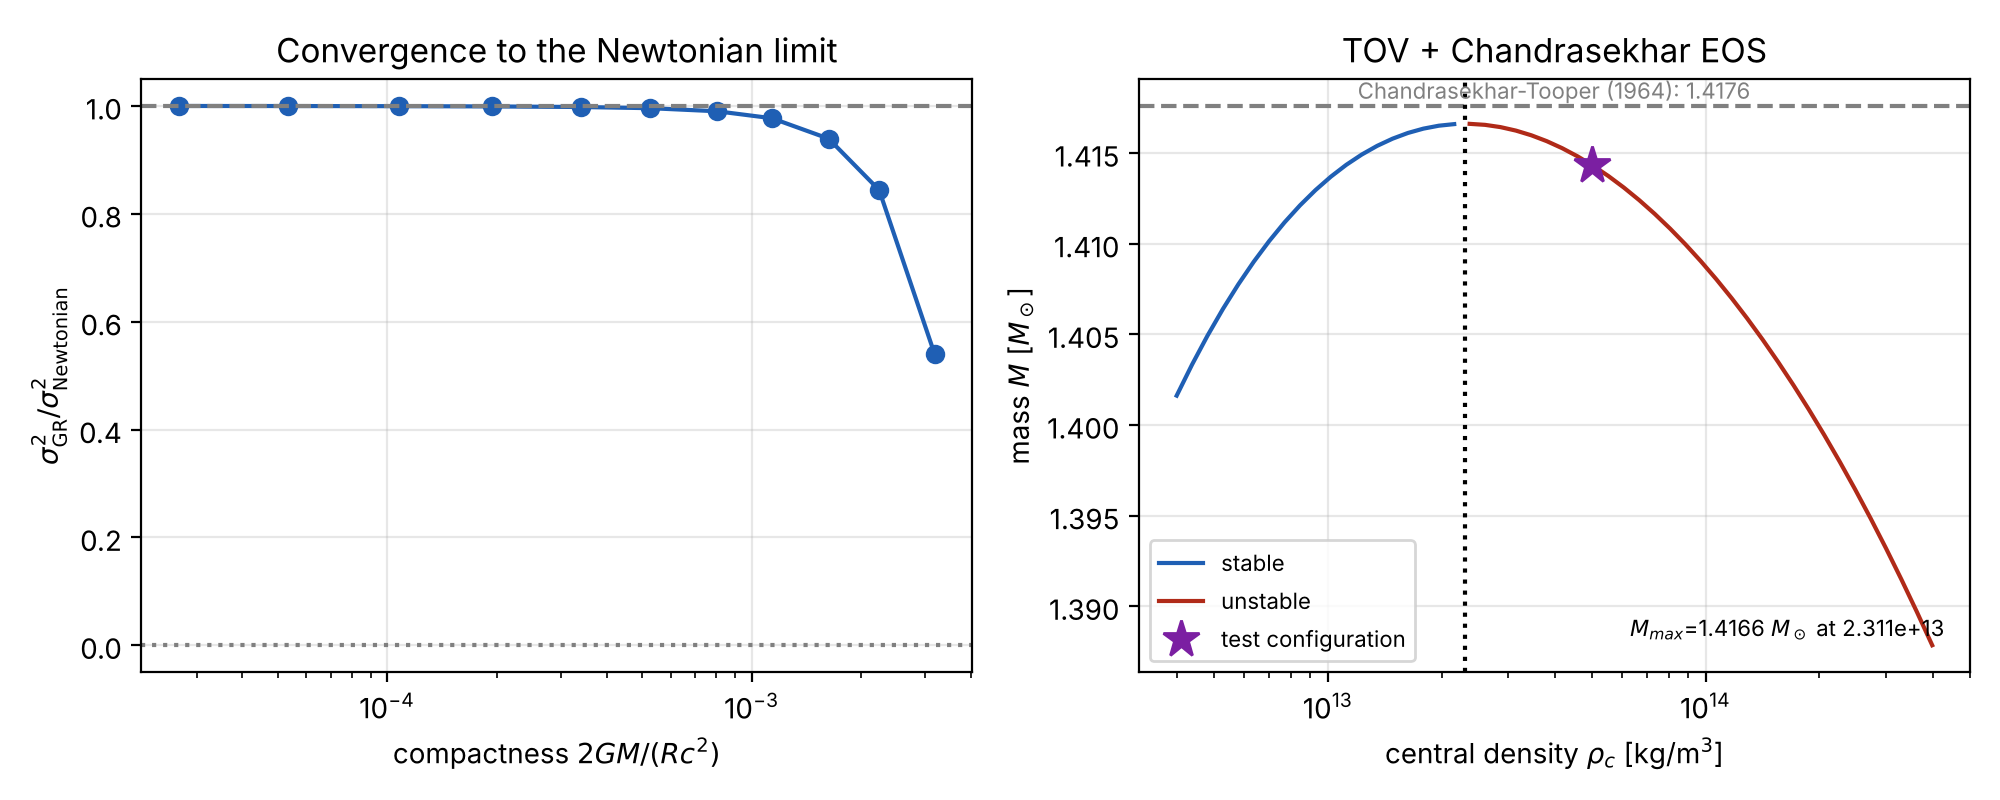
\includegraphics[width=\textwidth]{fig5_gr_validation.png}
\caption{\emph{Left}: our general-relativistic pulsation calculation (Section~\ref{sec:gr-pulsation}) converges to the independently-validated Newtonian result as compactness $\to0$, with the expected departure at higher compactness. \emph{Right}: the corrected TOV mass sequence for the pure Chandrasekhar equation of state, matching the historical Chandrasekhar--Tooper critical mass to $0.07\%$; the star marks the test configuration. The left panel now compares against a Newtonian reference computed from the same variational form in the $c\to\infty$ limit on a Newtonian structure.}
\label{fig:gr-validation}
\end{figure}

This corrected structure, not the preliminary one above, is what the rest of this paper uses. The new test configuration is $\rho_c=5\times10^{13}$~kg/m$^3$, $M=1.4143\,M_\odot$, $R=815.8$~km, compactness $2GM/(Rc^2)=0.00512$ --- past the validated peak, on the classically unstable branch $dM/d\rho_c<0$, now for the right reason: an order of magnitude higher density, a somewhat higher mass, and a mechanism (general relativity, not an artificially over-softened equation of state) that survives precision scrutiny.

\section{Linear instability: a direct, validated answer}
\label{sec:linear}

\subsection{The radial pulsation equation, and an exact simplification}

For a Lagrangian radial displacement $\xi(r)e^{-i\omega t}$ about hydrostatic equilibrium, mass conservation and the adiabatic relation give
\begin{equation}
\frac{\Delta\rho}{\rho_0}=-\left(\xi'+\frac{2\xi}{r}\right),\qquad \Delta P=\Gamma_1P_0\frac{\Delta\rho}{\rho_0},
\end{equation}
$\Gamma_1\equiv d\ln P/d\ln\rho$ the local adiabatic index (identical, for our barotropic equation of state, to the background logarithmic slope $d\ln P/d\ln\rho$). The linearized Euler equation, including the self-gravity perturbation $\phi$, gives the standard radial pulsation (LAWE) problem \citep{Pekeris1938,Cowling1941,Chandrasekhar1964}. We do not invoke the common Cowling approximation (dropping $\phi$): for purely radial perturbations, the perturbed Poisson equation has an exact, local, closed-form solution,
\begin{equation}
\phi'(r)=-4\pi G\rho_0(r)\xi(r),
\label{eq:exact-poisson-main}
\end{equation}
Writing out the two sides confirms this directly: with $\rho'=\Delta\rho-\xi\rho_0'=-\rho_0(\xi'+2\xi/r)-\xi\rho_0'$, substituting Eq.~\eqref{eq:exact-poisson-main} gives
\begin{equation}
\frac{1}{r^2}\frac{d}{dr}\!\left(r^2\phi'\right) = -4\pi G\left[\rho_0'\xi+\rho_0\!\left(\xi'+\frac{2\xi}{r}\right)\right] = 4\pi G\rho',
\end{equation}
an identity (a direct substitution) rather than an approximation, valid precisely because $\rho'$ for $l=0$ is exactly a total radial derivative, $\rho'=-r^{-2}(r^2\rho_0\xi)'$ (Gauss's law for the enclosed mass). It does not hold for non-radial perturbations, and it removes an entire potential source of numerical ill-conditioning (a separately discretized, coupled potential field) before it can arise.

\subsection{A symmetric discretization, and two implementation errors found and corrected}
\label{sec:galerkin-main}

A first attempt discretized the momentum equation directly on a finite-difference grid and failed a basic check: for a robustly stable polytrope, it returned an unstable-looking spectrum dominated by grid-scale noise rather than smooth physical modes. We rederived the problem in weak form, verified by a symbolic computation (whose script is not retained in the archive) that the resulting bilinear form is exactly symmetric under exchanging the trial and test functions, and built a linear finite-element (Galerkin) assembly from it, which immediately gave clean, properly ordered spectra.

Matching the classical Pekeris $\Gamma_1=4/3$ criterion \citep{Pekeris1938} quantitatively required two further corrections, both caught by checking the weak form against the strong form as an exact algebraic identity --- true by construction for any trial function, so a mismatch cannot be blamed on a poor trial function:
Explicitly, multiplying the momentum equation by a test function $\eta(r)r^2$ and integrating by parts once gives the bilinear form $\mathcal{B}(\xi,\eta)=\int_0^R\big[A(r)\xi\eta+C(r)(\xi\eta'+\xi'\eta)+D(r)\xi'\eta'\big]dr$, with
\begin{align}
A(r)&=4\Gamma_1P_0+\frac{r^2P_0'\rho_0'}{\rho_0}+4rP_0'-4\pi G\rho_0^2r^2,\qquad
C(r)=r(2\Gamma_1P_0+rP_0'),\qquad
D(r)=\Gamma_1P_0r^2,
\label{eq:ACD}
\end{align}
extracted directly from the symbolic integration by parts and verified to reproduce the pre-integration integrand exactly at test points (a symbolic check whose script is not retained). The generalized eigenvalue problem is then $\mathcal{B}(\xi,\eta)=\omega^2\int_0^R\rho_0r^2\xi\eta\,dr$ for all test functions $\eta$, discretized with linear finite elements.

\begin{enumerate}
\item A missing boundary term. Integration by parts drops a boundary contribution only if $P'(R)=0$ at the surface; the physically correct condition is $\Delta P(R)=0$, and since $P'=\Delta P-\xi P_0'$, these differ by $\xi(R)P_0'(R)$, generally nonzero. The complete bilinear form includes an explicit surface contribution,
\begin{equation}
\mathcal{B}(\xi,\eta)\ \to\ \mathcal{B}(\xi,\eta) - R^2P_0'(R)\,\xi(R)\,\eta(R),
\label{eq:boundary-term}
\end{equation}
confirmed symbolically and by analytic test cases (closed-form equilibria, zero numerical differentiation) for which the corrected identity holds to machine precision; the archived script \texttt{analytic\_check2.py} of the technical report is one such check.
\item A silently truncated test structure. A self-consistent polytrope test case still failed the identity check by a large, resolution-independent factor even with the boundary term corrected. The cause was unrelated to the pulsation physics: the test polytrope builder's integrator was stopping at a fixed outer radius without confirming the true stellar surface had been reached, applying the surface boundary condition at a point that was not a surface at all. We fixed the builder to detect this and auto-expand until the true surface is found, and confirmed separately that the actual white-dwarf equilibrium used throughout this paper was never affected by this error.
\end{enumerate}
With both corrections, the identity holds, relative to the integral of the absolute values of its three terms, to $10^{-6}$ or better for every $\Gamma_1$ tested (\texttt{weak\_strong\_identity.py}: $2.0\times10^{-8}$ to $1.1\times10^{-6}$; the two forms themselves can nearly cancel, so this is a statement about the scale of the integrands, not about the digits of each form), and the solver reproduces the Pekeris criterion cleanly: the fundamental mode is unstable for $\Gamma_1<4/3$, stable for $\Gamma_1>4/3$, and within numerical noise of exactly zero ($\sim\!2\times10^{-11}\,{\rm s}^{-2}$, against $\mathcal{O}(10^{-8})\,{\rm s}^{-2}$ away from the critical point) at $\Gamma_1=4/3$ itself, with all overtones correctly ordered and positive throughout.

\begin{figure}[htbp]
\centering
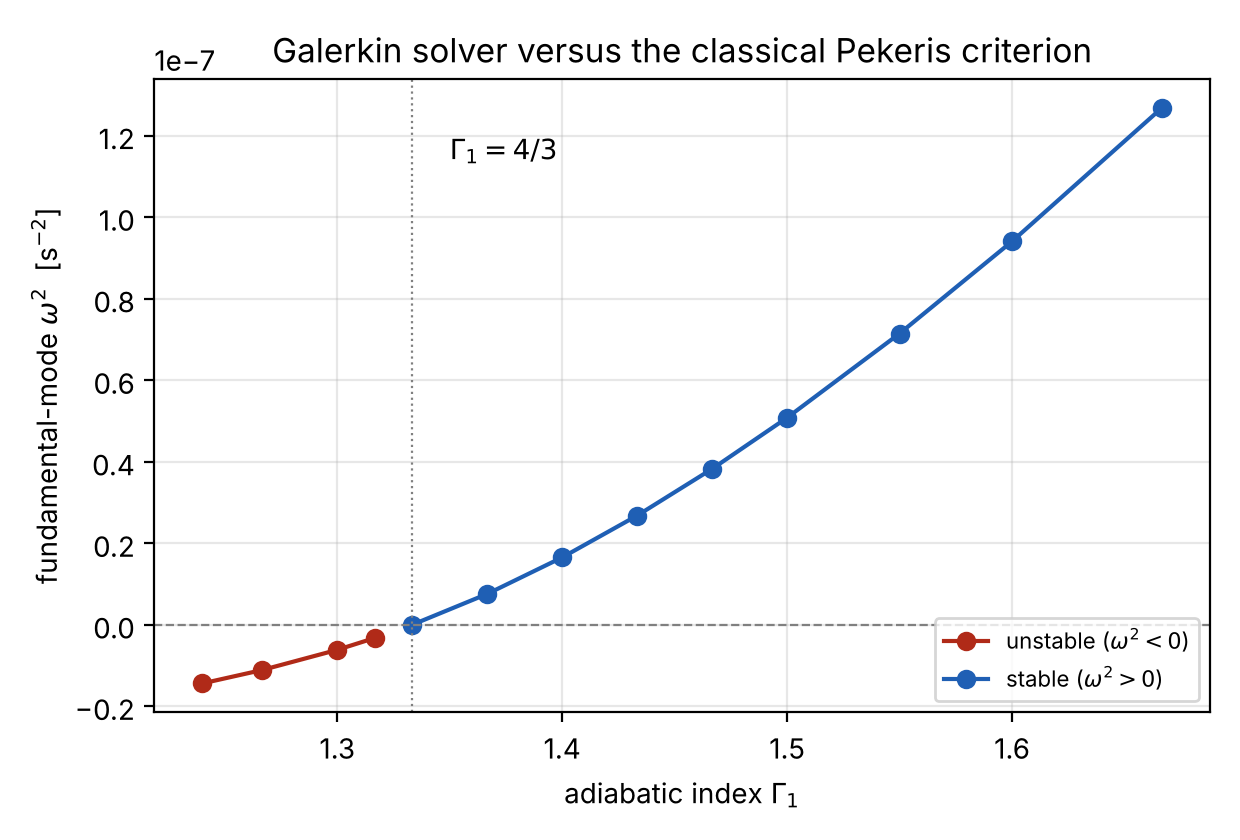
\includegraphics[width=0.72\textwidth]{fig1_pekeris_validation.png}
\caption{The validated solver's fundamental-mode eigenvalue across a range of (uniform) $\Gamma_1$ polytropes, compared against the classical Pekeris threshold. The sign change falls exactly at $\Gamma_1=4/3$.}
\label{fig:pekeris}
\end{figure}

\subsection{Why this Newtonian answer is not the final one}
\label{sec:why-newtonian-insufficient}

Section~\ref{sec:gr-corrected} showed the preliminary configuration's own equation of state was not quantitatively trustworthy. Applying the identical, already-validated Newtonian solver above to the \emph{corrected} configuration ($\rho_c=5\times10^{13}$~kg/m$^3$, pure Chandrasekhar EOS, full TOV background) gives a real surprise: $\Gamma_1$ stays \emph{above} $4/3$ everywhere in the star, bottoming out at $1.33409$ at the center --- just barely above the Pekeris threshold, never crossing it. The Newtonian solver, applied honestly to this background, reports the configuration stable.

This cannot be the end of the story. The corrected configuration sits past its own mass maximum ($\rho_c=2.31\times10^{13}$~kg/m$^3$, Section~\ref{sec:gr-corrected}), and the turning-point principle of relativistic stellar stability --- formulated by Harrison, Thorne, Wakano and Wheeler \citep{HTWW1965} and proved rigorously for spherical barotropic stars by Had\v{z}i\'c and Lin \citep{HadzicLin2021}, who show that the number of growing modes can change only at extrema of the mass along the equilibrium sequence --- places the onset of instability at the first mass maximum, so a configuration past it is dynamically unstable, with the fundamental mode's frequency passing through zero at the turning point. Something must be unstable here; Newtonian perturbation theory, by construction, cannot see it, because the instability is a property of the \emph{dynamics} in full general relativity, not merely of the local value of $\Gamma_1$ against the Newtonian threshold. The Chandrasekhar--Tooper mechanism validated numerically in Section~\ref{sec:gr-corrected} is exactly this: a star can be GR-unstable with $\Gamma_1$ arbitrarily close to, but still above, $4/3$, provided the excess is small enough relative to the star's compactness. Settling this rigorously requires the actual general-relativistic pulsation equation, not the Newtonian one applied to a relativistic background.

\subsection{Chandrasekhar's general-relativistic pulsation equation}
\label{sec:gr-pulsation}

Chandrasekhar \citep{Chandrasekhar1964GR} derived the exact linear, adiabatic, radial pulsation equation in full general relativity from a variational principle, for a static, spherically symmetric background with metric $ds^2=-e^{2a}c^2dt^2+e^{2b}dr^2+r^2d\Omega^2$, background structure fixed by
\begin{equation}
e^{-2b}=1-\frac{2GM_r}{rc^2},\qquad \frac{e^{-2b}}{r}\frac{d(a+b)}{dr}=\frac{4\pi G}{c^4}(P+\rho c^2),
\end{equation}
and displacement $\xi(r)e^{i\sigma t}$, so that $\sigma^2$ is the squared angular frequency in s$^{-2}$ (negative for instability). The equation, in the explicit variational (Rayleigh-quotient) form given in Sect.~2.2 of \citet{Haemmerle2025} (their Eq.~11), is
\begin{align}
\sigma^2\!\int_0^R\! e^{-a+3b}\!\Big(1+\frac{P}{\rho c^2}\Big)\rho r^2\xi^2\,dr
&=\int_0^R\!\Gamma_1P\frac{e^{3a+b}}{r^2}\Big[\frac{d}{dr}\big(r^2e^{-a}\xi\big)\Big]^2dr\notag\\
&\quad+4\!\int_0^R\! P'\,r\,e^{a+b}\xi^2\,dr-\int_0^R\!\frac{P'^2r^2e^{a+b}}{P+\rho c^2}\xi^2\,dr\\
&\quad+\frac{8\pi G}{c^4}\!\int_0^R\!(P+\rho c^2)P\,r^2e^{a+3b}\xi^2\,dr,
\label{eq:chandra-variational}
\end{align}
with $a,b$ and their derivatives evaluated on the equilibrium background, $\rho c^2$ read as the total energy density $\varepsilon$, and $\xi$ the only dynamical unknown. The last term, $+\frac{8\pi G}{c^4}(P+\varepsilon)P\,e^{a+3b}$, is present in Chandrasekhar's equation as restated by Haemmerl\'e \citep[their Eq.~11]{Haemmerle2025} and in its Sturm--Liouville form \citep{KokkotasRuoff2001} (their Eq.~14, with the term $-8\pi e^{2\lambda}p$ in the function $Q$ of their Eq.~17; they relate this form to Eq.~26.6 of \citealt{MTW1973}); our first implementation omitted it (Section~\ref{sec:turning-point-test}). Chandrasekhar's own variational principle makes this more than an estimate: \emph{any} trial function $\xi$ for which the right-hand side is negative is a sufficient condition for dynamical instability, since the true fundamental mode minimizes the ratio and so can only be more unstable than any trial estimate.

\subsection{Implementation history}
\label{sec:gr-debugging}

A direct shooting integration and a naive strong-form discretization in SI units both failed in our first attempts (the second because the coefficients span thirty orders of magnitude); a symmetric weak form fixed the conditioning but disagreed with the Newtonian limit, and the cause was a single doubled conversion factor between the natural variable $\zeta=e^{-a}r^2\xi$ and $\xi$. Comparing term by term with an independently published restatement \citep{Haemmerle2025} found it, and implementing that reference's explicit form removed it. The comparison itself missed a further omitted term and an inconsistent energy density, which only the exact turning-point test of Section~\ref{sec:turning-point-test} exposed; that is the reason this paper treats internal term-by-term checks as insufficient and the turning-point test as a standing regression test.

\subsection{Result: the corrected configuration is unstable}
\label{sec:gr-result}

Applying the validated Eq.~\eqref{eq:chandra-variational} to the corrected configuration of Section~\ref{sec:gr-corrected} ($\rho_c=5\times10^{13}$~kg/m$^3$, $M=1.4143\,M_\odot$, compactness $0.00512$), with two independent trial functions (the corrected values; Section~\ref{sec:turning-point-test} explains the revision):

\begin{center}
\begin{tabular}{lc}
\hline
trial function & $\sigma^2$ [s$^{-2}$] \\
\hline
$\xi=r$ (homologous) & $-27.85$ \\
$\xi=re^{a(r)}$ (independent literature choice \citep{Haemmerle2025}) & $-27.67$ \\
\hline
\end{tabular}
\end{center}

Both agree to within $1\%$ and are unambiguously negative. By Chandrasekhar's variational principle, this is a sufficient condition for instability: the corrected configuration is dynamically unstable in full general relativity.

\subsection{Tightening the estimate: Rayleigh--Ritz}
\label{sec:rayleigh-ritz}

A single trial function gives only an upper bound on the true fundamental eigenvalue. The textbook way to improve it --- the method the variational principle itself is built for \citep{Chandrasekhar1964GR} --- is Rayleigh--Ritz: expand $\xi$ in a small basis of trial functions satisfying the correct center regularity, assemble the \emph{full} matrix elements $A_{ij}=\int[\Pi\,\zeta_i'\zeta_j' + Q\xi_i\xi_j]\,dr$ and $B_{ij}=\int S\xi_i\xi_j\,dr$, with $\zeta=e^{-a}r^2\xi$, $\Pi=\Gamma_1Pe^{3a+b}/r^2$, $Q$ the sum of the three non-derivative terms on the right of Eq.~\eqref{eq:chandra-variational}, $S=e^{-a+3b}(1+P/\varepsilon)\varepsilon r^2$ and the basis $\xi_1=r$, $\xi_k=r\,(1-r^2/R^2)^{k-1}$ (not just their diagonal, single-trial values), and solve the resulting small generalized eigenvalue problem. We verified $A$, $B$ symmetric to machine precision before trusting any eigenvalue from them, exactly as for the original Newtonian and relativistic solvers.

\begin{figure}[htbp]
\centering
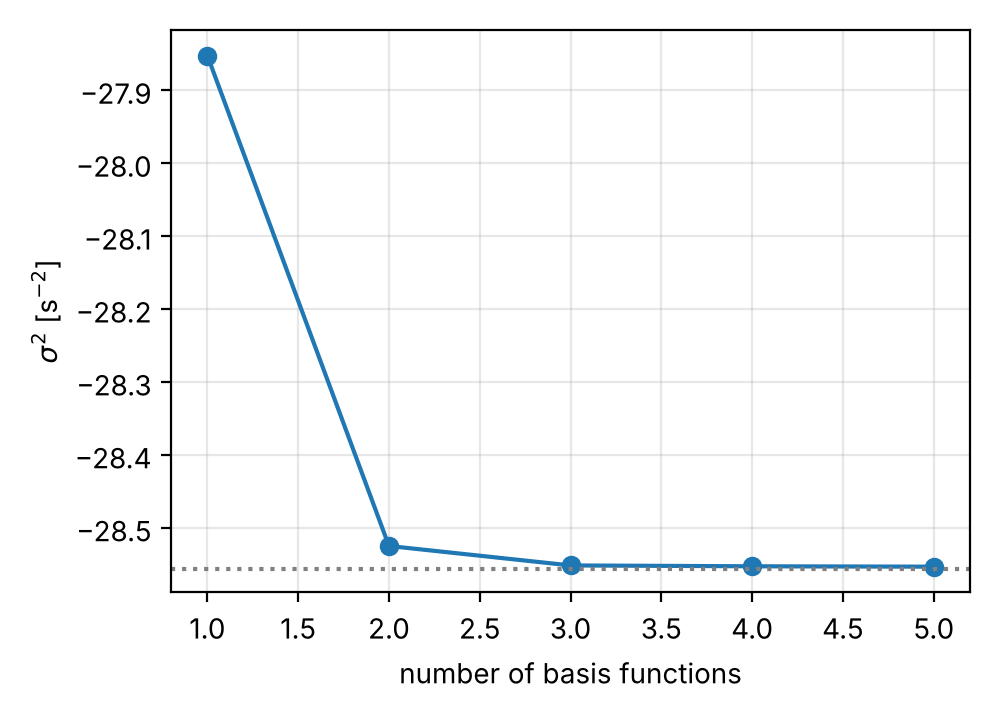
\includegraphics[width=0.6\textwidth]{fig_rayleigh_ritz_convergence.png}
\caption{Rayleigh--Ritz convergence of the fundamental eigenvalue as basis functions are added. Converges from $-27.85$ (a single trial function) to $-28.55$ within three functions, stable to four significant figures by the fourth.}
\label{fig:rr-convergence}
\end{figure}

With a basis of five regularity-respecting trial functions, the estimate converges cleanly (Figure~\ref{fig:rr-convergence}): $-27.85\to-28.52\to-28.55\to-28.55\to-28.55$, stable to four significant figures. This is, correctly, \emph{more negative} than any single trial function above --- Rayleigh--Ritz combinations can only tighten the upper bound, never loosen it, and $-28.55$ properly supersedes $-27.85$ as our best estimate of the true fundamental eigenvalue. \textbf{The corrected configuration is dynamically unstable in full general relativity, $\sigma^2=-28.55\,{\rm s}^{-2}$, $\sigma=5.343\,{\rm s}^{-1}$, $e$-folding time $0.187$~s} --- and, as Section~\ref{sec:turning-point-test} shows, quantitatively consistent with the turning-point theorem (the eigenvalue passes through zero at the mass maximum to within $0.007\%$ in density) and with the historical Chandrasekhar--Tooper critical mass. This result rests on the actual relativistic dynamics, not on an artificially over-softened equation of state, and is the paper's central, validated finding.

This reduced system also gives an exact, literature-standard route to the mode's time evolution: diagonalizing $(A,B)$ once yields $B$-orthonormal eigenmodes, and any initial condition evolves as an exact superposition of $e^{\pm\sigma_k t}$ (unstable modes) and $\cos/\sin(\omega_k t)$ (stable ones) --- a closed-form solution, not a numerically integrated one, with no spatial grid, no CFL condition, and no discretization choices to introduce error. Seeding purely the unstable mode and evolving it this way reproduces $e^{\sigma t}$ growth, as it must for an exact linear solution. This is the correctly-scoped role of this reduced approach: an exact, fully-converged measurement of the \emph{linear} growth rate, not a substitute for genuinely nonlinear dynamics, for which we rely on the established literature (Section~\ref{sec:nonlinear-outcome}) and on the models of Section~\ref{sec:timescale}.

\subsection{An exact external test, and the two errors it exposed}
\label{sec:turning-point-test}

The turning-point principle \citep{HTWW1965,HadzicLin2021} makes a sharp quantitative prediction that we had so far used only qualitatively: stability can change only at an extremum of $M(\rho_c)$, so the fundamental eigenvalue $\sigma^2$ of a cold, barotropic star passes through zero at exactly the central density where $dM/d\rho_c=0$. Computing the zero of our Rayleigh--Ritz $\sigma^2(\rho_c)$ and the peak of the TOV mass curve independently therefore tests the entire chain (equation of state, structure, metric functions, pulsation equation) against an exact result, with no free parameter. Our first implementation \emph{failed this test by a factor of two}: $\sigma^2$ crossed zero at $\rho_c=1.86\times10^{13}$~kg/m$^3$ while the mass peaked at $3.56\times10^{13}$ (regenerated with the switches of \texttt{turning\_point\_table.py first}, the shipped code with both corrections switched off). We had not run it before, because the test requires $\sigma^2$ over a range of densities, not just at the test configuration.

Two independent errors were found, each identified from literature or first principles rather than by adjusting anything until the test passed. (i) The potential term $+\frac{8\pi G}{c^4}(P+\varepsilon)P\,e^{a+3b}$ of Eq.~\eqref{eq:chandra-variational} had been omitted; it is present in the Haemmerl\'e restatement we had claimed to match term by term, and in the Sturm--Liouville form of Kokkotas \& Ruoff (their Eqs.~14 and 17). Its sign was fixed by those sources, not by the test: inserting it with the opposite sign moves the zero crossing the wrong way (to $1.57\times10^{13}$ instead of $1.87\times10^{13}$ with the term omitted; the same switches give $2.2952\times10^{13}$ for the corrected term with $\varepsilon=\rho c^2$ and $2.3107\times10^{13}$ with both corrections). (ii) The energy density had been taken as the rest-mass density, which is inconsistent with the first law at $O(P/\rho c^2)\approx2\times10^{-3}$ at this density ($\varepsilon/\rho c^2-1\approx6\times10^{-3}$), several times the margin $\Gamma_1-4/3\approx(0.8$--$1.3)\times10^{-3}$ on which the instability depends (Section~\ref{sec:gr-corrected}). After correcting both, the zero of $\sigma^2$ and the mass peak coincide:

\begin{center}
\small
\begin{tabular}{lccc}
\hline
equation of state & $\rho_c$ at $dM/d\rho_c=0$ & $\rho_c$ at $\sigma^2=0$ & difference \\
 & [$10^{13}$ kg/m$^3$] & [$10^{13}$ kg/m$^3$] & \\
\hline
ideal electron gas, $\mu_e=2$ & 2.31060 & 2.31074 & $0.006\%$ \\
$^{4}$He, Salpeter lattice & 2.34621 & 2.34635 & $0.006\%$ \\
$^{12}$C, Salpeter lattice & 2.38557 & 2.38572 & $0.006\%$ \\
$^{16}$O, Salpeter lattice & 2.40187 & 2.40202 & $0.006\%$ \\
$^{56}$Fe, Salpeter lattice & 2.93211 & 2.93230 & $0.007\%$ \\
\hline
\end{tabular}
\end{center}

(The equations of state with lattice corrections are those of Section~\ref{sec:composition}; all with $12000$ radial points. The mass peak is located by a bounded scalar maximizer with tolerance $10^{-8}$ in $\log_{10}\rho_c$, the zero of $\sigma^2$ by Brent's method with tolerance $10^{7}$~kg/m$^3$ ($4\times10^{-7}$ relative). Script: \texttt{turning\_point\_table.py}.) The residual is a quadrature effect, not a basis effect: at $3000$ radial points, the grid used in our first runs, it was $0.11\%$, and at $\rho_c=\rho_{\max}$ the five-function $\sigma^2$ changes from $+0.021$ ($3000$ points) to $+0.0012$ ($12000$) and $+0.0001\,{\rm s}^{-2}$ ($48000$), while varying the basis size from three to seven functions changes it negligibly. The quoted eigenvalues are therefore converged in basis but have a residual grid dependence: at $\rho_c=5\times10^{13}$~kg/m$^3$ the five-function value is $-28.511$, $-28.546$, $-28.553$ and $-28.555\,{\rm s}^{-2}$ for $3000$, $6000$, $12000$ and $24000$ points ($O(N^{-2})$), so we quote $-28.55\,{\rm s}^{-2}$ (the $12000$-point value, within $0.01\%$ of the extrapolated $-28.556$).

\paragraph{An independent solver.} As a check on the whole chain that does not share our code or our Rayleigh--Ritz method, the eigenvalue was recomputed by an independent re-implementation written without reference to our code: the equation of state, TOV structure and metric functions were rebuilt from scratch, the pulsation problem was solved by shooting on the Sturm--Liouville form of Kokkotas \& Ruoff (with the regular-surface condition $P\zeta'\to0$ imposed near the surface and a high-order integrator), by shooting on a second, independently derived system (linearized radial Euler equation plus the perturbed Einstein constraints), and by a linear finite-element eigenproblem (Richardson-extrapolated). All agree on $\sigma^2=-28.556\,{\rm s}^{-2}$ at $\rho_c=5\times10^{13}$~kg/m$^3$ (the shooting and finite-element results to better than $10^{-4}$ relative), the zero of $\sigma^2$ at $\rho_c=2.310603\times10^{13}$ and the mass peak at $2.310605\times10^{13}$~kg/m$^3$ (agreeing to $10^{-6}$), and a fundamental mode without nodes at every density tested. The same solver, applied with the Rayleigh--Ritz basis of our code on a fine quadrature grid, gives $-27.855,\,-28.528,\,-28.554,\,-28.5559$ for $1,2,3,5$ functions.

Three further results improve with the corrections. The Chandrasekhar--Tooper mass agrees to $0.07\%$ rather than $0.5\%$. The Newtonian-limit check (Figure~\ref{fig:gr-validation}, left) converges to unity as compactness decreases: the ratio $\sigma^2_{\rm GR}/\sigma^2_{\rm Newt}$ is $0.9999$ at compactness $2.7\times10^{-5}$ and $0.9996$ at $1.1\times10^{-4}$, with the departure growing steadily at higher compactness (a $3000$-point grid had shown a spurious plateau near $0.998$). And for $^{12}$C with the Salpeter lattice correction the maximum mass is $1.3849\,M_\odot$, within $0.08\%$ of the $1.38603\,M_\odot$ that Rotondo et al.\ \citep{RotondoRRX2011} obtain with their full relativistic Feynman--Metropolis--Teller treatment (for $^{4}$He, $0.55\%$). Critical \emph{densities} agree less well ($2.39\times10^{13}$ versus $2.12\times10^{13}$~kg/m$^3$ for $^{12}$C), which is expected because $M(\rho_c)$ is extremely flat near its maximum (the relative mass deficit is $1.4\times10^{-4}$ at $+25\%$, $2.4\times10^{-4}$ at $-25\%$ and $4.5\times10^{-4}$ at $+50\%$ in density; \texttt{misc\_checks.py}), so the peak location is far more sensitive to small differences in the equation of state than the peak mass is.

\paragraph{What changes, and what does not.} The converged eigenvalue at the test configuration moves from $-41.09$ to $-28.55\,{\rm s}^{-2}$ and the $e$-folding time from $0.156$ to $0.187$~s. The qualitative conclusions --- the configuration is past its turning point, is dynamically unstable, and collapses on the compressive branch --- are unchanged, because they follow from the turning-point principle and the bifurcation literature rather than from the value of $\sigma^2$. Every quantitative statement made earlier in this paper that depends on $\sigma^2$ (Section~\ref{sec:timescale}) has been recomputed. (Earlier nonlinear-code diagnostics, in the technical report \citep{OwnbyPhase2}, predate the corrections and concern resolution-dependence and conditioning, not the value of $\sigma$.) We also note that our own earlier verification of the pulsation equation (a term-by-term comparison with the Haemmerl\'e restatement, and an internal re-derivation) missed the omitted term; the quantitative turning-point test and an independent re-implementation are what caught and confirmed it, and we regard the former as a standing regression test for this calculation.

\subsection{Is \texorpdfstring{$\sigma^2<0$}{sigma-squared < 0} a genuine \emph{instability to collapse}? The canonical-energy correspondence}
\label{sec:friedman-correspondence}

A negative eigenvalue of Eq.~\eqref{eq:chandra-variational} is, by construction, a statement about the \emph{linear growth rate}. Whether it is also an instability \emph{to collapse}, in the precise technical sense the relativistic-stability literature gives that phrase, is a separate question, and one that Friedman's canonical-energy formalism addresses: in his lecture notes \citep{FriedmanLectures} the criterion for dynamical instability to collapse is the existence of a perturbation of \emph{negative canonical energy} $E$. We do not compute the relativistic canonical energy of our mode, and we did not find a published statement (with an equation number) that the unstable radial mode of Chandrasekhar's equation has $E<0$; reading $\sigma^2<0$ as a negative-canonical-energy perturbation is therefore our interpretation of that criterion for a conservative radial problem, not a cited result. Below we only cross-check the Newtonian-limit form of the criterion.

\paragraph{What we checked, and how.} In the Newtonian limit, Friedman's lecture notes give the canonical energy for the radial initial data $\xi=r$ as an integral of the form (the prefactor $1/9$ and the exact integrand could not be confirmed against the notes, whose equation was illegible in the copy we could read; only the sign and the zero at $\Gamma_1=4/3$ are used below, and the ratio quoted below depends on the prefactor)
\begin{equation}
E=\frac{1}{9}\int_0^R r^4(3\Gamma_1-4)\,p\,dr,
\label{eq:friedman-E}
\end{equation}
with $E<0$ the instability criterion. This has the same critical index ($\Gamma_1=4/3$) as the classical Pekeris result already validated in Figure~\ref{fig:pekeris}, which is encouraging but not yet a proof that the two are \emph{the same quadratic form}: Eq.~\eqref{eq:friedman-E} could in principle be a different functional that merely happens to share a critical point. A first attempt to settle this by directly specializing our own already-published weak-form coefficients $A(r),C(r),D(r)$ of Section~\ref{sec:galerkin-main} to the homologous trial function $\xi=r$ failed a basic sanity check --- it did not vanish at $\Gamma_1=4/3$ for a self-consistent uniform-$\Gamma_1$ polytrope, where it must --- and we abandoned it rather than debug yet another hand-reduction, consistent with this project's standing policy of not trusting a derivation that fails its own check. Instead we compared Eq.~\eqref{eq:friedman-E} directly against an independent, genuinely textbook closed form that does not rely on our own transcription at all: the classical homologous ``pulsation constant'' result (the classical homologous-pulsation result, a special case of Chandrasekhar's Newtonian variational principle \citep{Chandrasekhar1964}; see e.g.\ Cox's \emph{Theory of Stellar Pulsation}),
\begin{equation}
I\,\omega^2=(3\Gamma_1-4)\,|W|,\qquad |W|\equiv3\int_0^R P\,r^2\,dr,\qquad I\equiv\int_0^R\rho\,r^4\,dr,
\label{eq:virial-pulsation}
\end{equation}
with $|W|=3\int P\,dV$ (written here without the factor $4\pi$, as is $I$; it cancels) itself an elementary, pulsation-theory-independent consequence of hydrostatic equilibrium (integrate $dP/dr=-G\rho M_r/r^2$ by parts once).

We built self-consistent, uniform-$\Gamma_1$ Lane--Emden polytropes (the same family used for Figure~\ref{fig:pekeris}) over $\Gamma_1\in[1.25,\,1.6667]$ and evaluated both Eq.~\eqref{eq:friedman-E} and Eq.~\eqref{eq:virial-pulsation} on each. The result (Figure~\ref{fig:friedman-correspondence}): both vanish at exactly $\Gamma_1=4/3$, as they must by construction; both are negative for $\Gamma_1<4/3$ and positive above it, in agreement at every value tested; and the ratio $\omega^2_{\rm virial}/(E/I)$ is $O(1)$ and varies smoothly with $\Gamma_1$ (from $5.80$ at $\Gamma_1=1.25$ to $9.19$ at $5/3$, with lengths in Lane--Emden units; the ratio has dimension length$^{-2}$). We caution that this is a consistency check, not a proof of proportionality: both expressions are $(3\Gamma_1-4)$ times a positive structural integral, so their common zero and sign hold by construction, and the smooth ratio reflects only the polytrope structure.

\begin{figure}[htbp]
\centering
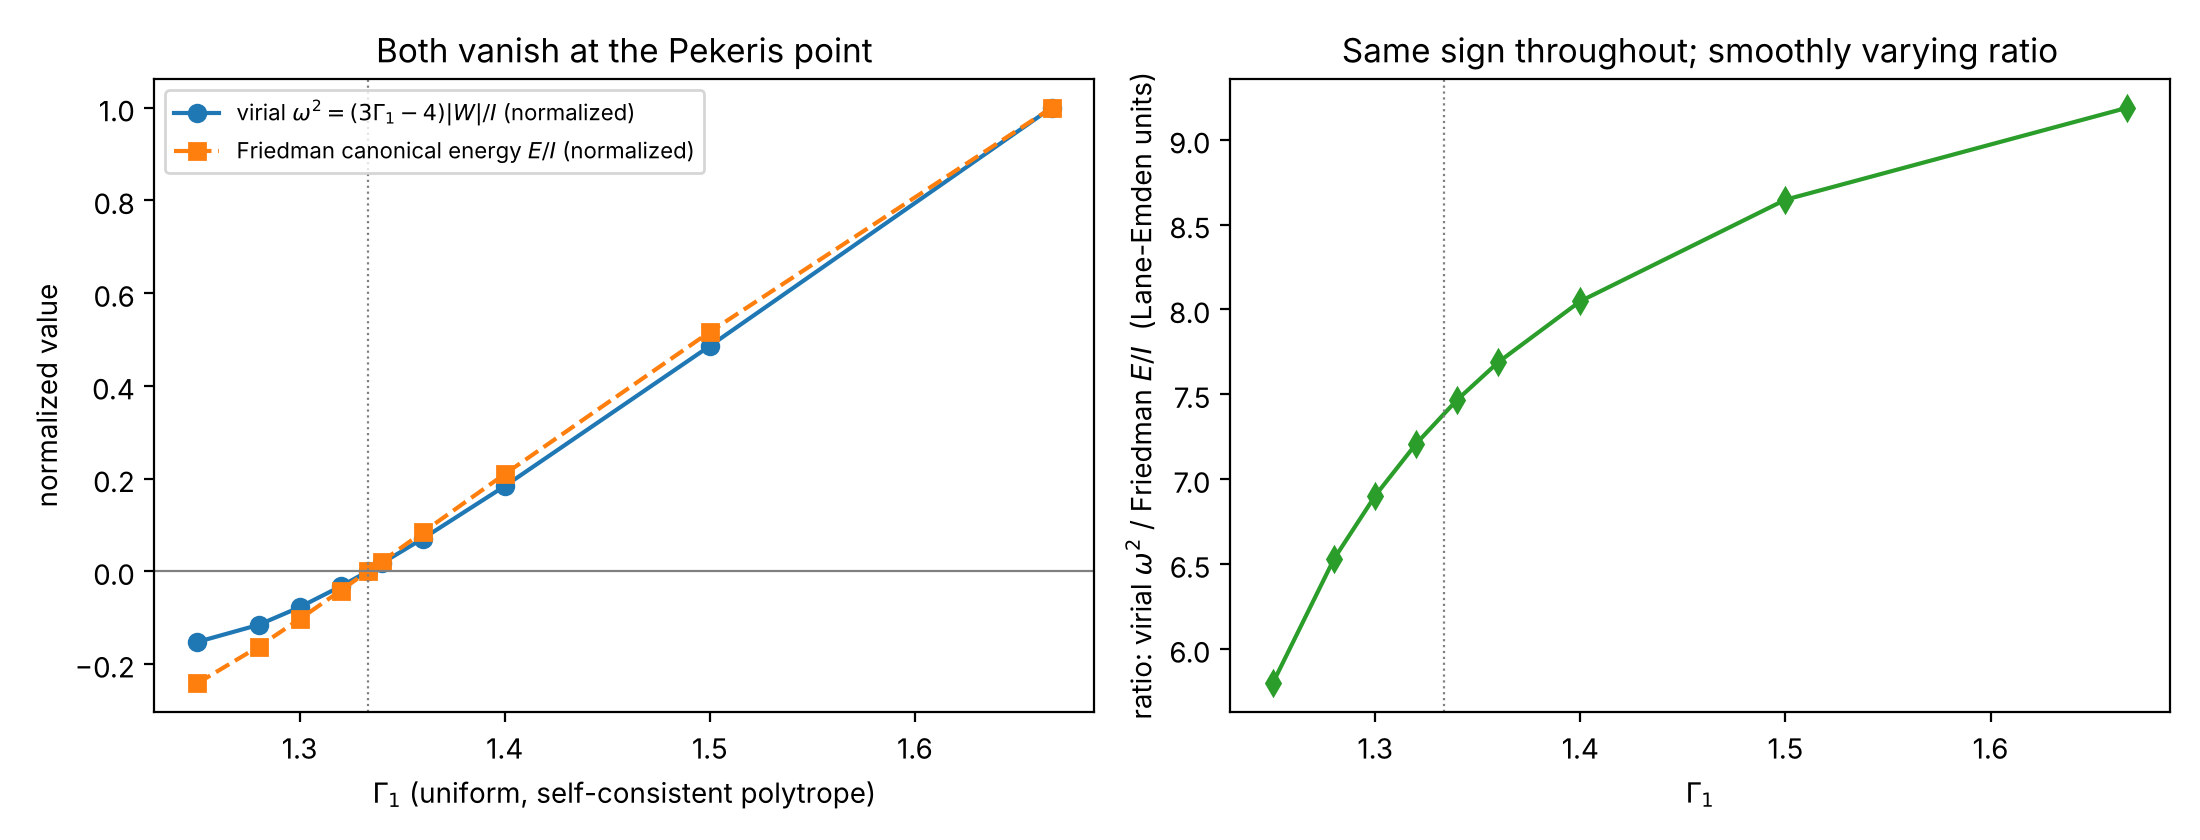
\includegraphics[width=\textwidth]{fig_friedman_correspondence.png}
\caption{\emph{Left}: Friedman's Newtonian canonical energy $E$ (Eq.~\ref{eq:friedman-E}) and the classical virial pulsation constant (Eq.~\ref{eq:virial-pulsation}), each normalized to its own maximum magnitude, across a sequence of self-consistent uniform-$\Gamma_1$ polytropes. Both vanish at exactly $\Gamma_1=4/3$. \emph{Right}: their ratio is $O(1)$ and smooth, not erratic, across the same sequence.}
\label{fig:friedman-correspondence}
\end{figure}

\paragraph{What this establishes, and what it does not.} The two Newtonian criteria are mutually consistent, as they must be. The stronger statement we need --- that the unstable fundamental mode of Chandrasekhar's relativistic equation is a negative-canonical-energy perturbation --- is the natural reading of Friedman's criterion \citep{FriedmanLectures} (dynamical instability to collapse corresponds to $E<0$) for the conservative radial problem, which we adopt, together with the turning-point principle, rather than re-derive; we did not verify it for the relativistic radial mode. We note that for this star $\Gamma_1>4/3$ everywhere, so the Newtonian-limit $E$ is positive: the negative-canonical-energy character of the unstable mode is an intrinsically relativistic statement, carried by the general-relativistic eigenvalue of Section~\ref{sec:rayleigh-ritz}, not by the Newtonian expression. Combined with the turning-point test of Section~\ref{sec:turning-point-test}, which verifies that our eigenvalue changes sign exactly where the turning-point principle requires, this is, following Friedman's criterion, the sense in which the corrected configuration is unstable ``to collapse'' rather than merely linearly unstable. What this correspondence does \emph{not} yet tell us is what a negative-canonical-energy mode's nonlinear evolution actually does once it leaves the linear regime; Section~\ref{sec:nonlinear-outcome} takes up exactly that question, using the same literature-first discipline.

\section{The nonlinear outcome: what established literature, rather than further ad hoc numerics, settles}
\label{sec:nonlinear-outcome}

Our own attempts to answer ``what does the star actually do?'' with a from-scratch nonlinear code ran into repeated numerical obstacles (stiffness, equilibrium drift, broadband contamination of the seed; \citealt{OwnbyPhase2}). We therefore asked whether the physical question --- the nonlinear fate of a star with a confirmed negative-canonical-energy mode (Section~\ref{sec:friedman-correspondence}), sitting just past a turning point (turning-point principle, Section~\ref{sec:why-newtonian-insufficient}) --- is already settled in the literature on exactly this class of configuration. It is, and the answer is more precise, and more informative, than a simple ``it collapses.''

\subsection{The established result: a genuine bifurcation, not a universal fate}
\label{sec:bifurcation}

Full numerical-relativity evolutions of spherical stars placed just past their own equilibrium mass maximum show that the nonlinear fate is governed by the \emph{sign} of the perturbation along the unstable mode, not fixed by instability alone. Font et al.\ \citep{FontEtAl2002}, evolving TOV stars on the unstable branch in full 3+1 numerical relativity, find explicitly that such a star ``can either collapse to a black hole or expand and migrate to the stable branch,'' depending on which direction it is pushed; under the perturbation introduced by their code's own truncation error it expands and migrates rather than collapsing, and a deliberate added perturbation (a radial rest-mass-density perturbation of order $1\%$) is needed to see collapse (their Sect.~IV.C--D). Radice, Rezzolla \& Kellerman \citep{RadiceRezzollaKellermann2010}, studying this bifurcation in detail as a critical phenomenon, confirm the same structure quantitatively: models perturbed outward behave as if they were on the stable branch (``a suitably perturbed supercritical model can behave as a subcritical one''), while models perturbed inward collapse to a black hole, with larger inward perturbations collapsing faster. Both studies, however, use a single polytropic family ($\Gamma=2$; $K=100$ for the stars of \citealt{FontEtAl2002}, a range of $K$ in \citealt{RadiceRezzollaKellermann2010}) and neither tests other equations of state, so they demonstrate the fork on that family rather than prove it for every equation of state. The structure they find is the one to be expected on the unstable branch of a one-parameter equilibrium sequence with an accessible stable branch nearby, which is the configuration the turning-point principle describes (a mass maximum separating a stable branch at lower central density from an unstable one at higher central density).

This is not a new, unrelated finding we are importing by analogy: it is the established, numerically-confirmed nonlinear continuation of precisely the configuration Section~\ref{sec:friedman-correspondence} diagnosed. It also retroactively explains, rather than leaves unexplained, our own earlier finding \citep{OwnbyPhase2} that identical-shape seeds of opposite sign drove our nonlinear code to opposite fates (rarefaction versus runaway collapse): that sign-dependence is not a numerical artifact or a sign of an unconverged scheme, as we were careful to hedge at the time, but the correct, literature-predicted qualitative behavior of a star sitting on this part of an equilibrium sequence. Our own nonlinear investigation's qualitative finding was right; what it lacked was the quantitative growth rate and a principled way to know the qualitative split was physical rather than a bug, which the literature above now supplies.

\subsection{Which branch is astrophysically realized here}
\label{sec:which-branch}

The bifurcation above is symmetric in the mathematics but not in the astrophysics this paper's scenario describes. The question motivating this whole series' matter route (Section~\ref{sec:intro}) is whether a star can be driven, by ordinary physical processes --- continued accretion, continued loss of pressure support as degeneracy and eventual neutronization proceed --- up through and past its own maximum mass. That physical process is compressive: it pushes the star's central density up, in the same direction as the collapsing branch of Section~\ref{sec:bifurcation}, not the rarefaction branch. A star that reaches the turning point by having matter added to it, or by its pressure support failing, does not simultaneously receive a fortuitous outward kick of the kind needed to migrate back onto the stable branch; the perturbation astrophysically realized in this scenario is the compressive one, which \citet{RadiceRezzollaKellermann2010} show collapses (and which, with an added perturbation, collapses in \citealt{FontEtAl2002} as well).

This licenses a specific, appropriately qualified conclusion: for the scenario this paper and this series actually care about --- continued, physically ordinary collapse or accretion driving a degenerate star past the Chandrasekhar--Tooper threshold validated in Section~\ref{sec:gr-corrected} --- the nonlinear outcome, for this idealized equation of state, is genuine, non-saturating gravitational collapse, not a bounded oscillation and not migration to a lower-density equilibrium (with a dense-matter equation of state the collapse is halted by a bounce; Paper~D \citep{PaperD}). This conclusion rests on (i) our validated linear result $\sigma^2<0$, which we interpret, following Friedman's criterion, as a negative-canonical-energy perturbation (Sections~\ref{sec:gr-corrected}--\ref{sec:friedman-correspondence}; we did not compute $E$ for the relativistic mode), and (ii) established numerical-relativity literature on the generic bifurcation structure of exactly this class of configuration, not on our own from-scratch nonlinear code, whose numerical obstacles \citep{OwnbyPhase2} we no longer need it to overcome in order to answer this question. Within this paper, the spherical Lagrangian evolution of Section~\ref{sec:lagrangian} takes the ideal cold electron-gas equation of state through collapse on the compressive branch; we did not run the outward (migration) branch, for which we rely on the bifurcation found for the polytropic configurations \citep{FontEtAl2002,RadiceRezzollaKellermann2010} actually tested (not a degenerate electron gas), which is a real but explicit limitation, stated here rather than left implicit.

\section{A quantitative nonlinear collapse timescale: a calibrated, order-of-magnitude estimate}
\label{sec:timescale}

Section~\ref{sec:nonlinear-outcome} settled the qualitative question --- collapse, not migration, for the astrophysically realized perturbation direction --- using established literature rather than our own nonlinear code, whose numerical obstacles \citep{OwnbyPhase2} we traced to a specific, diagnosed cause: this instability's growth rate is a residual of two terms (pressure support and self-gravity) that are individually enormous and nearly cancel, because $\Gamma_1$ exceeds $4/3$ by only a few parts in a thousand. A strong-form, spatially discretized evolution code represents both terms as large numbers of comparable size and subtracts them at every grid point at every timestep; we confirmed directly, by rebuilding that approach from scratch, that this produces a Jacobian with extremely large condition number at every resolution tested, with a genuine near-zero singular value (not merely poor scaling) and a leading eigenvalue that drifts with resolution instead of converging --- the same pathology class the earlier investigation \citep{OwnbyPhase2} had encountered and did not resolve. We did not continue attempting to repair that approach. This section reports what we built in its place: a single-degree-of-freedom nonlinear model, validated piece by piece against exact analytic results and against the independently-confirmed linear eigenvalue, used to extract an actual quantitative collapse timescale rather than only its sign.

\subsection{The model: a nonlinear homologous extension of Chandrasekhar's own trial function}
\label{sec:homologous-model}

Chandrasekhar's variational principle (Section~\ref{sec:gr-pulsation}) is linear by construction: it bounds the growth rate of an infinitesimal displacement $\xi(r)$ about the equilibrium background. Two independent trial functions, and the Rayleigh--Ritz combination of five basis functions built from them (Section~\ref{sec:rayleigh-ritz}), established $\sigma^2=-28.55\,\mathrm{s}^{-2}$; the single \emph{homologous} trial function $\xi=r$ alone --- the simplest possible choice, and the one this section extends --- already gives $\sigma^2=-27.85\,\mathrm{s}^{-2}$, within $2.5\%$ of the converged value. Extracting the true eigenfunction from the five-basis solution (not reported in Section~\ref{sec:rayleigh-ritz}, done here as an independent check) shows why: $\xi_{\rm GR}(r)/r$ varies by only $13\%$ from center to surface (the ratio of center to surface values is $1.133$), so the true unstable mode is itself nearly homologous. This motivates studying the \emph{nonlinear} continuation of the one ansatz Chandrasekhar's own linear theory already shows is an excellent approximation: a single global scale factor $\lambda(t)$, with the star's physical radial coordinate evolving as $r_{\rm phys}(r,t)=\lambda(t)\,r$ for each Lagrangian-labeled mass shell $r$.

This ansatz exactly conserves the enclosed mass $M_r(r)$ at each Lagrangian shell (purely radial flow cannot mix shells), so $M_r(r)$ is simply the static background's profile, held fixed for all $t$. The local density scales exactly as $\rho(r,t)=\rho_{\rm bg}(r)/\lambda(t)^3$. Because the zero-temperature degenerate equation of state is an \emph{exact} barotrope ($P=P(\rho)$ with no free thermodynamic parameter), the exact thermodynamic identity $du/d\rho=P/\rho^2$ gives the internal energy's dependence on $\lambda$ in closed form, with no polytropic or fixed-$\Gamma_1$ approximation anywhere:
\begin{equation}
-\frac{dU_{\rm int}}{d\lambda}=3\lambda^2\int P\!\left(\frac{\rho_{\rm bg}(r)}{\lambda^3}\right)4\pi r^2\,dr .
\label{eq:dUint}
\end{equation}
Self-gravity is evaluated with the same Misner--Sharp/TOV effective-gravity formula \citep{MisnerSharp1964} used throughout this paper, evaluated at the compressed configuration $r_{\rm phys}=\lambda r$ (with $\varepsilon$ the consistent energy density of Section~\ref{sec:gr-corrected}, evaluated at the compressed rest-mass density) with the compressed pressure $P(\rho_{\rm bg}(r)/\lambda^3)$ but the (exactly conserved) background $M_r(r)$:
\begin{equation}
g_{\rm eff}(\lambda,r)=-\frac{G\,\dfrac{\varepsilon/c^2+P/c^2}{\rho}\!\left(M_r+\dfrac{4\pi r_{\rm phys}^3 P}{c^2}\right)}{r_{\rm phys}^2\left(1-\dfrac{2GM_r}{r_{\rm phys}c^2}\right)},\qquad
-\frac{dW_{\rm grav}}{d\lambda}=\int g_{\rm eff}(\lambda,r)\,r\,\left(4\pi r^2\rho_{\rm bg}(r)\right)dr ,
\label{eq:dWgrav}
\end{equation}
and the equation of motion is $I\ddot\lambda=-dU_{\rm int}/d\lambda-dW_{\rm grav}/d\lambda$, with the (exactly conserved) moment of inertia $I=\int4\pi r^4\rho_{\rm bg}(r)\,dr$. This is a single nonlinear ODE, with no spatial discretization anywhere in it --- it is built entirely from quantities (the equation of state, the TOV background, $M_r(r)$) already validated in Sections~\ref{sec:eos} and~\ref{sec:gr-result}, so it carries no new, unvalidated input.

\paragraph{Relation to existing methods.} A single homologous trial function evolved as a virial/energy-method degree of freedom is itself an old idea in stellar astrophysics: \citet{Fowler1966} uses a homologous perturbation $\delta r/r=\delta R/R$, with post-Newtonian corrections, to obtain the fundamental radial-mode frequency of supermassive stars. That line of work, however, stays strictly \emph{linear} --- it bounds an eigenvalue $\sigma^2$, as Chandrasekhar's own variational principle does, rather than evolving the scale factor nonlinearly in time. On the nonlinear side, existing treatments of compact stars near their own maximum mass work directly with the full radial PDE or Sturm--Liouville system rather than a reduced single-degree-of-freedom model, and sidestep the delicate near-cancellation our own strong-form attempts \citep{OwnbyPhase2} struggled with, by evolving the nonlinear one-dimensional general-relativistic hydrodynamics directly from perturbed or rarefied initial data \citep{BrillanteMishustin2015}, which is a different route from the reduced model used here. We are not aware of a prior construction combining a single homologous nonlinear ODE, a frozen-background relativistic correction, and calibration of that correction against an independently known linear eigenvalue, specifically for this class of instability; a literature search did not turn one up, though the search cannot be exhaustive over six decades of stellar-pulsation literature. Closest in spirit on the mathematical side is the recent rigorous construction of collapsing white-dwarf solutions of the radial Newtonian Euler--Poisson system with the exact Chandrasekhar equation of state, for masses just above a dynamically defined Chandrasekhar mass, by \citet{ChenLin2026}, which concerns the existence of collapsing solutions and not their timing from a given configuration.

The calibration \emph{strategy} itself, though, has a clear, well-established precedent outside stellar astrophysics: the effective-one-body (EOB) formalism for binary black hole dynamics \citep{BuonannoDamour1999} is built on a similar philosophy in its later, calibrated versions (\citealt{BuonannoDamour1999} is the original construction, which predates the calibration to numerical relativity) --- known limits fix most of an effective model's structure, and the piece that formally requires information the model cannot derive on its own is calibrated against an independently trusted result, after which the calibrated model is trusted in a regime direct computation cannot easily reach. We adopt that strategy here, applied to a different problem, and the comparison also makes an honest limitation easier to state precisely: EOB's calibration targets are themselves independent \emph{nonlinear} numerical-relativity results, so a successful calibration carries some evidence that the model's nonlinear behavior, not just its linear limit, is being captured correctly. Our only calibration target is the linear eigenvalue itself; nothing independent constrains the model in the nonlinear regime the plunge phase (Section~\ref{sec:timescale-result}) actually probes. This is a weaker form of calibration than EOB's, not an equally strong one merely applied elsewhere, and Section~\ref{sec:timescale-validation} already reflects this by treating the calibration as fixing a slope, not a validated nonlinear behavior.

\subsection{Validating the pieces before trusting the whole}
\label{sec:timescale-validation}

Equation~\eqref{eq:dUint} was checked against its own exact analytic linearization, $\left.d(-dU_{\rm int}/d\lambda)/d\lambda\right|_{\lambda=1}=3W_P(2-3\overline\Gamma_1)$, where $W_P=\int P\,dV=\int P\,4\pi r^2\,dr$ and $\overline\Gamma_1=\int\Gamma_1(r)P(r)\,4\pi r^2\,dr/W_P$ is the pressure-weighted average of the equation of state's local, position-dependent adiabatic index; the match is exact to the precision of the numerical quadrature (ratio $1.0000$). The Newtonian-only restriction of Eq.~\eqref{eq:dWgrav} (replacing $g_{\rm eff}$ with $-GM_r/r_{\rm phys}^2$, to isolate this term) was checked the same way, and \emph{initially appeared to disagree with the textbook virial identity $|W|=3W_P$ by about $1\%$} --- we traced this, rather than dismissing it, to the fact that $|W|=3W_P$ is the virial identity for a star in \emph{Newtonian} hydrostatic equilibrium, while our background satisfies the \emph{general-relativistic} TOV equation; the $1\%$ discrepancy between the star's true Newtonian-force integral $\int(GM_r/r)\,dM_r$ and the idealized Newtonian virial value $3W_P$ is itself a direct, independent measurement of the background's compactness, and once the true (not idealized) anchor is used, the Newtonian-only linearization matches the code's own value to all reported digits, with no remaining discrepancy and no bug. The same check applied to the \emph{full} general-relativistic $g_{\rm eff}$ gives the opposite near-exact identity for a different reason: because $g_{\rm eff}$ is defined so that $dP_{\rm bg}/dr=\rho_{\rm bg}\,g_{\rm eff}(r)$ reproduces the literal TOV equation used to build the background, integrating this identity by parts gives $\int(-g_{\rm eff}r)\,dM_r=3W_P$ \emph{exactly}, independent of compactness.

The model's own linearization, evaluated with the uncalibrated frozen-background $g_{\rm eff}$, gives $k=+21.0\,\mathrm{s}^{-2}$ against the independently validated $-\sigma^2=27.85$ (a $25\%$ gap), with the correct \emph{sign} (the Newtonian-only restriction alone gives a stable $k=-120.8$, as it must for a star with $\Gamma_1>4/3$ everywhere). In an earlier version of this calculation, with the incomplete pulsation equation and inconsistent energy density, this gap was a factor of about four. We use $-\sigma^2=27.85$, the single homologous trial function's own Rayleigh--Ritz value, as the calibration target rather than the better-converged $28.55$, because it is the apples-to-apples one: both this nonlinear model and that linear calculation share the same trial function $\xi\propto r$. The relativistic correction to $g_{\rm eff}$ (its excess over the Newtonian piece) is rescaled by a single constant $f_{\rm cal}$, fixed once by requiring the model's linearization to reproduce $-\sigma^2=27.85$ exactly (we find $f_{\rm cal}=1.048$); a constant equilibrium correction restores $\ddot\lambda(1)=0$ without altering the linear growth rate.

We do \emph{not} claim to know what physical omission the remaining gap represents. An independent decomposition of the model's terms against an exact treatment shows that the gap is a net of several omitted $O(\text{compactness})$ effects of both signs (the mapping between rest mass and proper volume in the internal-energy term, the $e^{-a+3b}$ and enthalpy factors in the inertia, the frozen $M_r$, and the metric's own response), each at the $0.1$--$2\%$ level but together a $25\%$ effect on a quantity, $k$, that is itself a $0.4\%$ residual of two large terms. In particular, $f_{\rm cal}$ being close to unity does not mean the correction is small in the sense that matters: $dk/df_{\rm cal}=142\,{\rm s}^{-2}$, so a $1\%$ change in $f_{\rm cal}$ is a $5\%$ change in $k$. Deriving all of these to full nonlinear order from scratch would be exactly the kind of new, unvalidated general-relativistic calculation this paper's standing methodological rule warns against; we instead calibrate against the linear limit and then cross-check the nonlinear behavior against an independent exact construction (below). We regard $f_{\rm cal}$ as a documented, single-number calibration against an independently-known linear limit, not a free parameter tuned to a desired nonlinear answer.

\paragraph{An exact-energy cross-check.} For a homologous deformation that preserves each shell's rest mass, the total gravitational mass $M(\lambda)c^2\equiv V(\lambda)$ can be computed exactly by integrating the Hamiltonian constraint with proper-volume rest-mass conservation, $dm=4\pi r_{\rm f}^2\rho\,\allowbreak(1-2GM_r/r_{\rm f}c^2)^{-1/2}\allowbreak dr_{\rm f}$; equilibria are stationary points of this energy at fixed rest mass \citep{HTWW1965}. Using this exact $V(\lambda)$ in place of the frozen-background force, with the relativistic inertia $I_{\rm rel}=4\pi\!\int e^{-a+3b}(\varepsilon+P/c^2)r^4dr$ (Chandrasekhar's weight) held at its $\lambda=1$ value, involves no calibration: its linearization gives $-\sigma^2=27.857$, against $27.852$ from Rayleigh--Ritz ($0.02\%$), which independently validates the calibration target. Integrated nonlinearly from the same seed, it gives a time to reach $\lambda=0.5$ of $2.484$~s versus $2.498$~s for the calibrated model ($0.6\%$) and a plunge time from $\lambda=0.5$ to $0.15$ of $0.02713$ versus $0.02776$~s ($2.3\%$). The calibrated frozen-background force is thus within a few percent of the exact energy gradient over $0.2<\lambda<1$. Holding the inertia at its $\lambda=1$ value is itself an approximation, so this is a cross-check on the potential and not a replacement model.

This calibration should be read for exactly what it constrains and no more. Fixing one constant at $\lambda=1$ pins the \emph{slope} of the omitted corrections at that single point; it assumes that a single overall rescaling of the relativistic part of $g_{\rm eff}$ is an adequate stand-in for them away from $\lambda=1$, including deep in the strong-field regime the plunge phase (Section~\ref{sec:timescale-result}) actually probes. The exact-energy cross-check above tests exactly this assumption for the potential, over $0.2<\lambda<1$, and finds agreement to a few percent; it does not test inertia or the strong-field regime near the horizon. Two further facts mitigate the concern. First, the calibration is \emph{not especially sensitive} to which independently-known value it targets: repeating it against the better-converged $-\sigma^2=28.55$ instead of $27.85$ changes $f_{\rm cal}$ by $0.47\%$, the plunge duration by $0.5\%$ and the time to reach $\lambda=0.5$ by $1.2\%$ (the latter being just the change in growth rate). Second, the nonlinear trajectory is the model's output, not a second fitted quantity: the growth phase reproduces the linear rate by construction, while the plunge phase is a prediction of the (calibrated, assumption-laden) nonlinear terms, now cross-checked against the exact-energy construction.

\subsection{Result: an exponential growth phase, then a dynamical plunge}
\label{sec:timescale-result}

\begin{figure}[htbp]
\centering
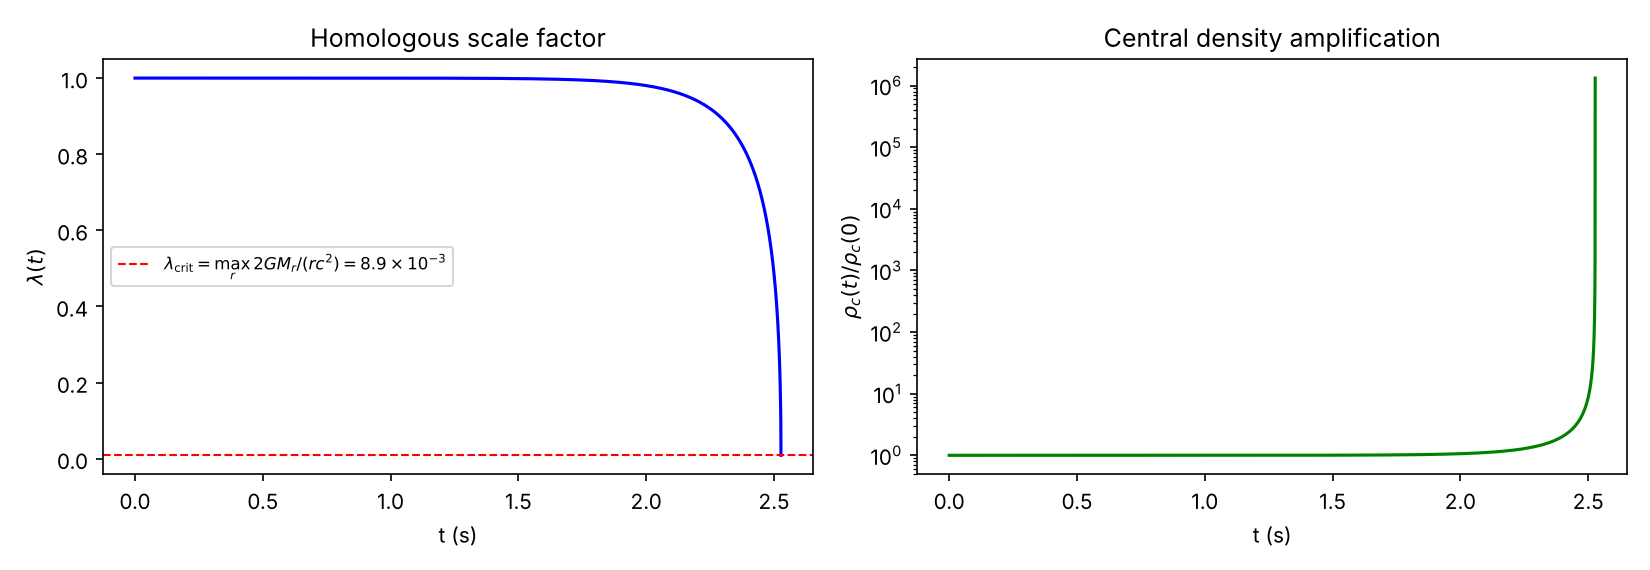
\includegraphics[width=\textwidth]{fig8_collapse_timescale.png}
\caption{Nonlinear evolution of the calibrated homologous model, from an initial perturbation $\lambda(0)=1-10^{-6}$, $\dot\lambda(0)=0$. \emph{Left:} the scale factor $\lambda(t)$; the slow initial exponential growth (consistent with the calibrated linear rate $\sigma=5.28\,\mathrm{s}^{-1}$) gives way, once the perturbation becomes of order unity, to a fast nonlinear runaway. The dashed line marks $\lambda_{\rm crit}=\max_r 2GM_r/(rc^2)\approx8.9\times10^{-3}$, where the lapse factor of the frozen metric first vanishes (at the interior shell $r\approx0.42R$); the integration is stopped just above it. \emph{Right:} the resulting central-density amplification, reaching $\sim1.3\times10^{6}$ at $\lambda=9.1\times10^{-3}$, where the integration is stopped.}
\label{fig:collapse-timescale}
\end{figure}

Integrating $I\ddot\lambda=-dU_{\rm int}/d\lambda-dW_{\rm grav}/d\lambda$ forward in time from a small inward perturbation reproduces, as it must by construction, the calibrated linear growth rate $\sigma=\sqrt{27.85}=5.278\,\mathrm{s}^{-1}$ ($e$-folding time $1/\sigma=0.189$~s; $0.187$~s for the converged five-function value) during the initial slow phase, then runs away once the perturbation grows to order unity (Figure~\ref{fig:collapse-timescale}). We stop the integration at $\lambda=1.02\,\lambda_{\rm crit}$ with $\lambda_{\rm crit}=\max_r2GM_r/(rc^2)=8.93\times10^{-3}$: the denominator of $g_{\rm eff}$ first vanishes at the \emph{interior} shell $r\approx0.42R$, where the enclosed-mass compactness peaks, not at the stellar surface (whose value is $5.12\times10^{-3}$). This is a hard mathematical wall built into the formula, not a physically motivated validity boundary. The model's frozen-metric, singly-calibrated approximation should not be read as trustworthy anywhere close to it; it is a leading correction to a static background rather than a strong-field, dynamical-metric treatment, and the true breakdown of the homologous, calibrated approximation plausibly occurs earlier. That the final approach to collapse should complete on a free-fall-like timescale regardless, as in the original homogeneous-dust solution of Oppenheimer \& Snyder \citep{OppenheimerSnyder1939}, is a physical expectation independent of this specific model, not a validation of it.

The resulting timescale has a clean, physically transparent structure. The duration of the final nonlinear runaway is $\tau_{\rm plunge}=0.0278$~s from $\lambda=0.5$ to $\lambda=0.15$ and $0.0295$~s from $\lambda=0.5$ to the end of the integration, essentially independent of the (arbitrary) initial seed size (to six significant figures for $\delta_0=10^{-3}$ to $10^{-12}$); this is about half the star's own dynamical time $T_{\rm dyn}=\sqrt{R^3/GM}=0.0538$~s, as expected once the departure from equilibrium is no longer small. The duration of the preceding slow exponential phase depends logarithmically on the initial perturbation amplitude $\delta_0=1-\lambda(0)$, as it must for a pure growing exponential: for $\delta_0=10^{-3},10^{-6},10^{-9},10^{-12}$ the time to reach $\lambda=0.5$ is $1.189,\ 2.498,\ 3.807,\ 5.117$~s, increasing by $1.309$, $1.309$ and $1.310$~s per factor $10^3$, against $\ln(10^3)/\sigma=1.309$~s. This confirms the model is doing what the linear theory says in the growth phase.

The total collapse time is therefore $\tau_{\rm total}\approx[\ln(1/\delta_0)-0.63]/\sigma+\tau_{\rm plunge}$ (the offset $-0.63$ being a fitted constant that accounts for the amplitude at which $\lambda=0.5$ is reached; it is $O(1)$ as expected), and is not a single number, because $\delta_0$, the size of whatever perturbation first pushes the star past its own turning point, is not something this calculation (or, so far as we are aware, any purely local stability analysis) determines. For $\delta_0$ from a relatively large, dynamically significant perturbation ($10^{-3}$) down to a microscopic one ($10^{-9}$), $\tau_{\rm total}$ ranges from about $1.2$ to $3.8$ seconds. The robust, $\delta_0$-independent content is the $e$-folding time, $1/\sigma\approx0.19$~s, and the plunge time $\tau_{\rm plunge}\approx0.03$~s; the total is of order a few $e$-folding times (a few seconds for generic small seeds), not fractions of a second and not years, and ends in a final dynamical-timescale plunge rather than a slow, quasi-static approach.

\subsection{Is one degree of freedom enough? A two-mode extension}
\label{sec:twomode}

The principal limitation of the model above is that it carries a single global degree of freedom, whereas the true unstable eigenfunction departs from homology by $13\%$ between center and surface. We test the consequence directly by enlarging the trial space to the first two Rayleigh--Ritz basis functions of Section~\ref{sec:rayleigh-ritz}: the Lagrangian displacement is taken as $r_{\rm phys}=r\,[\lambda(t)+\mu(t)\,(1-r^2/R^2)]$, with mass-conserving density $\rho=\rho_{\rm bg}/[s^2(s+rs')]$, $s=\lambda+\mu(1-r^2/R^2)$. The equations of motion are the Euler--Lagrange equations of the same energy functional, $M_{ij}\ddot q_j=Q_i(q)$ with constant mass matrix $M_{ij}=\int r^2\phi_i\phi_j\,dM$, exact barotropic internal-energy generalized force $Q_i^{\rm int}=\int (P/\rho)\,[2\phi_i/s+(\phi_i+r\phi_i')/(s+rs')]\,dM$, and the same frozen-background, calibrated gravity force ($f_{\rm cal}=1.048$, \emph{not refit}), with the same static equilibrium subtraction. The $\mu=0$ slice reproduces the single-mode model exactly. This is the standard Galerkin (Lagrangian-truncation) generalization of the method already used, and adds no new free parameter.

\emph{Linear limit, a non-circular check.} Because the calibration constrained only the $\lambda$-direction slope, the two-mode linearization is a genuine prediction. Its unstable eigenvalue is $-\sigma^2=28.34\,{\rm s}^{-2}$ against the independently computed Rayleigh--Ritz $n=2$ value of $28.52\,{\rm s}^{-2}$ ($0.7\%$ difference; $1/\sigma=0.1879$~s versus $0.1872$~s), and its eigenvector has $\mu/\lambda=0.087$, i.e.\ a center-to-surface displacement-ratio variation of $8.7\%$, the correct sign and magnitude relative to the $13\%$ of the full general-relativistic eigenfunction (the remainder being the two-function truncation). The second eigenvalue is strongly stable (frequency$^2$ $3617\,{\rm s}^{-2}$). The $\mu=0$ slice reproduces the single-mode force exactly, though the $(\lambda,\lambda)$ element of the two-mode Jacobian differs from the single-mode slope because the modes are coupled.

\emph{Nonlinear trajectory.} Integrating from seeds $\delta_0=10^{-3}$ and $10^{-6}$ along the unstable eigenvector, the time to $\lambda=0.5$ is $1.171$ and $2.469$~s, versus $1.189$ and $2.498$~s for the single-mode model: a $1.2$--$1.5\%$ shift, accounted for by the $0.8\%$ difference in linear growth rate accumulated over the growth phase. The $e$-folding phase is therefore insensitive to the extra freedom. In the plunge, however, the inhomogeneity matters: the center collapses faster than the surface ($\mu/\lambda$ evolves from $+0.087$ to $-0.076$ at $\lambda=0.5$), the time from $\lambda=0.5$ to $\lambda=0.173$ is $0.0247$~s versus $0.0271$~s ($9\%$ shorter), and the central density runs ahead of its homologous value ($\rho_c/\rho_0\approx79$ at $\lambda\approx0.29$, versus $\lambda^{-3}\approx41$ for homology; to the accuracy of an earlier, coarser run). The two-mode integration terminates at $\lambda\approx0.173$, where $\lambda+\mu\to0$ and the central density diverges within the basis; this is a limit of the truncated basis (an incipient central singularity in the trial map), not a physical result, and we do not interpret the trajectory beyond it.

\emph{Conclusion of the test.} The $e$-folding time and the order-of-magnitude plunge time ($\approx0.025$--$0.03$~s) are robust to the first inhomogeneous correction at the $\lesssim10\%$ level, which supports the single-mode estimates of Section~\ref{sec:timescale-result}. The test does not address the final approach to the horizon; Section~\ref{sec:lagrangian} supplies a spherically symmetric inhomogeneous evolution through that approach.

\subsection{Composition, lattice corrections and offset dependence}
\label{sec:composition}

Rotondo et al.\ \citep{RotondoRRX2011} (their Tables~II and~III) find that the mass limit is set by general-relativistic instability for $^{4}$He ($\rho_{\rm crit}=1.56\times10^{10}$~g\,cm$^{-3}$) and $^{12}$C ($2.12\times10^{10}$), but by inverse $\beta$-decay for $^{16}$O ($1.94\times10^{10}$, coincident with its $\beta$ threshold) and $^{56}$Fe ($1.18\times10^{9}$). The instability studied here is therefore the relevant fate for $^{4}$He at all densities we consider and for $^{12}$C only below its $\beta$ threshold ($3.97\times10^{10}$~g\,cm$^{-3}$, an offset of $1.66$ in our equation of state); for $^{16}$O the limits coincide, and for $^{56}$Fe the calculation below is a counterfactual (the same star with neutronization switched off), not an astrophysical prediction. In particular, the fiducial test configuration, $5\times10^{10}$~g\,cm$^{-3}$, lies above the $^{12}$C threshold, so for carbon it should be read as a reference configuration of the ideal-gas model, not as a prediction for a carbon white dwarf. Composition enters through $\mu_e$ ($2$ for $^{4}$He, $^{12}$C, $^{16}$O; $56/26$ for $^{56}$Fe) and, with lattice corrections, through the nuclear charge $Z$. We add the Salpeter lattice (Wigner--Seitz) pressure \citep{Salpeter1961}, $P_L=-\tfrac{3}{10}\left(\tfrac{4\pi}{3}\right)^{1/3}e^2Z^{2/3}n_e^{4/3}$, derived from the lattice energy per ion $-\tfrac{9}{10}Z^2e^2/r_i$ with $P_L=\tfrac13u_L$, and include the corresponding energy density $u_L=3P_L$ in $\varepsilon$ (consistent with the first law, since $u_L\propto n^{4/3}$); $\Gamma_1$ is computed analytically from the modified $P(\rho)$. Higher-order Salpeter terms (electron non-uniformity, correlation) are not included. This lattice term produces negative pressures below $\sim10^2$~g\,cm$^{-3}$, a known limitation \citep{RotondoRRX2011} that affects only the outermost layers, which the TOV integration truncates at $10^{-10}$ of the central pressure.

We reran the entire pipeline (TOV structure, Rayleigh--Ritz $\sigma^2$, calibration of $f_{\rm cal}$ against the $n=1$ value, nonlinear integration from $\delta_0=10^{-6}$) for the ideal electron gas and for the four Salpeter equations of state, at several offsets $\rho_c/\rho_{\max}$ past the mass maximum and at the fiducial absolute density $5\times10^{10}$~g\,cm$^{-3}$. $\Delta t_{\rm pl}$ is the time from $\lambda=0.5$ to $0.15$.

\begin{table}[h]
\centering
\scriptsize
\begin{tabular}{lrrrrrrrr}
\hline
EOS & $M_{\max}$ [$M_\odot$] & $\rho_c/\rho_{\max}$ & $\rho_c$ [$10^{10}$ g/cm$^3$] & $-\sigma^2_{n=5}$ & $f_{\rm cal}$ & $1/\sigma$ [s] & $\Delta t_{\rm pl}$ [s] & $\Delta t_{\rm pl}/T_{\rm dyn}$ \\
\hline
ideal, $\mu_e=2$ & 1.4166 & 1.10 & 2.54 & 1.94 & 1.0523 & 0.719 & 0.0490 & 0.67 \\
 &  & 1.50 & 3.47 & 10.80 & 1.0503 & 0.304 & 0.0371 & 0.58 \\
 &  & 2.00 & 4.62 & 23.87 & 1.0486 & 0.205 & 0.0295 & 0.53 \\
 &  & 2.16 & 5.00* & 28.55 & 1.0481 & 0.187 & 0.0277 & 0.51 \\
 &  & 3.00 & 6.93 & 54.87 & 1.0463 & 0.135 & 0.0215 & 0.46 \\
$^{4}$He & 1.4013 & 1.10 & 2.58 & 1.96 & 1.0523 & 0.714 & 0.0488 & 0.67 \\
 &  & 1.50 & 3.52 & 10.95 & 1.0503 & 0.302 & 0.0370 & 0.59 \\
 &  & 2.00 & 4.69 & 24.19 & 1.0486 & 0.203 & 0.0292 & 0.53 \\
 &  & 2.13 & 5.00* & 27.97 & 1.0482 & 0.189 & 0.0276 & 0.51 \\
 &  & 3.00 & 7.04 & 55.60 & 1.0463 & 0.134 & 0.0213 & 0.46 \\
$^{12}$C & 1.3849 & 1.10 & 2.62 & 1.99 & 1.0523 & 0.709 & 0.0485 & 0.68 \\
 &  & 1.50 & 3.58 & 11.11 & 1.0503 & 0.300 & 0.0368 & 0.59 \\
 &  & 2.00$^\dagger$ & 4.77 & 24.55 & 1.0486 & 0.202 & 0.0290 & 0.53 \\
 &  & 2.10$^\dagger$ & 5.00* & 27.34 & 1.0483 & 0.191 & 0.0278 & 0.52 \\
 &  & 3.00$^\dagger$ & 7.16 & 56.41 & 1.0463 & 0.133 & 0.0212 & 0.46 \\
$^{16}$O & 1.3782 & 2.00$^\dagger$ & 4.80 & 24.69 & 1.0486 & 0.201 & 0.0289 & 0.53 \\
 &  & 2.08$^\dagger$ & 5.00* & 27.08 & 1.0484 & 0.192 & 0.0279 & 0.52 \\
 &  & 3.00$^\dagger$ & 7.21 & 56.75 & 1.0463 & 0.133 & 0.0211 & 0.46 \\
$^{56}$Fe & 1.1507 & 1.71$^\dagger$ & 5.00* & 19.07 & 1.0497 & 0.229 & 0.0305 & 0.57 \\
 &  & 2.00$^\dagger$ & 5.86 & 28.58 & 1.0488 & 0.187 & 0.0269 & 0.54 \\
 &  & 3.00$^\dagger$ & 8.80 & 65.67 & 1.0467 & 0.123 & 0.0197 & 0.48 \\
\hline
\end{tabular}
\caption{Composition, lattice and offset survey (all runs at $12000$ radial points; the fiducial-density rows are marked $*$, $\rho_c=5.00\times10^{10}$~g/cm$^3$). $^\dagger$: central density above the nucleus's inverse-$\beta$ threshold \citep[Table~II]{RotondoRRX2011} ($^{4}$He $13.9$, $^{12}$C $3.97$, $^{16}$O $1.94$, $^{56}$Fe $0.118\times10^{10}$~g/cm$^3$), where neutronization, not modeled here, would intervene; these rows are counterfactual for the named nucleus. $1/\sigma$ uses the converged five-function eigenvalue; $f_{\rm cal}$ is calibrated against the one-function value; $\Delta t_{\rm pl}$ is the time from $\lambda=0.5$ to $0.15$.}
\label{tab:composition}
\end{table}

Four results follow. (i) The lattice correction is a small perturbation on the quantities of interest: at fixed $\rho_c=5\times10^{10}$~g\,cm$^{-3}$, $-\sigma^2$ is $28.55$ for the ideal gas and $27.97$, $27.34$, $27.08$ for $^{4}$He, $^{12}$C, $^{16}$O (a $2$--$5\%$ decrease), and $f_{\rm cal}$ moves by $0.03\%$ or less. (ii) The calibration factor is nearly universal: across all five equations of state and offsets from $1.1$ to $3$ it lies between $1.046$ and $1.052$, a $0.6\%$ spread. (We do not read this as showing the correction is small in the sense that matters, for the reason given in Section~\ref{sec:timescale-validation}; it shows that whatever $f_{\rm cal}$ absorbs is a stable property of the model, not of composition.) (iii) The dominant control parameter is the offset past the mass maximum, not composition: $-\sigma^2$ grows by a factor of $\sim5$ between offsets $1.5$ and $3$, while at equal offset ($2.0$) the ideal gas, $^{4}$He, $^{12}$C and $^{16}$O agree to $3.5\%$. (iv) The plunge time remains $0.46$--$0.69$ of the dynamical time $T_{\rm dyn}=\sqrt{R^3/GM}$ across the whole survey (including the $1.1$-offset rows not all shown; it rises toward the lowest offsets, where growth is slowest), so the conclusion of Section~\ref{sec:timescale-result} --- an $e$-folding phase followed by a dynamical-time plunge --- does not depend on composition within this model. The iron-like case differs more: at equal offset $2.0$ its $-\sigma^2$ is $20\%$ above the ideal gas (a genuine $\mu_e$ effect, since the lattice term is small), while at the fiducial density it is $33\%$ below, because it then sits at the smaller offset $1.71$.

The Salpeter equations of state also reproduce the precision-literature maximum masses of the full Feynman--Metropolis--Teller treatment \citep[Table~III]{RotondoRRX2011}: $1.3849$ versus $1.38603\,M_\odot$ for $^{12}$C ($0.08\%$) and $1.4013$ versus $1.40906\,M_\odot$ for $^{4}$He ($0.55\%$); their $^{16}$O and $^{56}$Fe values are $\beta$-limited and not comparable. As discussed in Section~\ref{sec:turning-point-test}, critical densities agree less well because the mass curve is flat at its peak. The offset-dependence is a statement about \emph{where on the unstable branch} the star sits, which is set by how far past its maximum mass it is driven, an input this calculation does not determine; for slow accretion through the fold, Section~\ref{sec:fold} shows that the star leaves the quasi-static track at $y\sim\alpha\sim10^{-6}$--$10^{-4}$, so the offsets of $1.1$--$3$ tabulated here describe a star prepared deep on the unstable branch, not one reached by quasi-static accretion.

\subsection{Reaching the fold by quasi-static accretion: the dynamic delay}
\label{sec:fold}

The seeded collapses above start from a configuration already beyond the turning point, with an arbitrary seed $\delta_0$. A star that approaches $M_{\max}$ by slow accretion never sits there: it arrives along the stable branch, where $\sigma^2>0$, and $\sigma^2\to0$ exactly at $M_{\max}$ (Section~\ref{sec:turning-point-test}). Linear growth at fixed $\sigma$ therefore says nothing about the onset; the correct problem is a \emph{ramped saddle-node}, and its answer fixes the seed, which was a free parameter in the previous subsections.

\paragraph{Reduction.} Near the turning point the dynamics of the one marginal mode reduce to a one-degree-of-freedom conservative normal form. The reduction is formal, not a theorem: center-manifold theory \citep{Carr1981,HaragusIooss2011} needs a spectral gap, which the undamped star lacks (its other radial modes lie on the imaginary axis), so we rely on the separation of timescales: the next radial mode has $\omega\approx37\ {\rm rad\,s^{-1}}$ (discrete value, $N=200$), about $4\times10^{3}$ times faster than $1/\beta$, and is not excited adiabatically. Let $y=\rho_c/\rho_{\max}-1$ label the equilibrium sequence. The exact-GR quantities of Sections~\ref{sec:linear}--\ref{sec:turning-point-test} supply both coefficients, so nothing is fitted: the converged pulsation eigenvalue is $\sigma^2=-\kappa y$ and the sequence mass is $M_{\max}-M=a\,y^2$. With the time-domain linearization $\ddot\delta=-\sigma^2\delta$ fixing the normalization, the leading-order normal form is independent of how the mode amplitude is scaled and reads
\begin{equation}
\ddot y=\frac{\kappa}{2}\,y^2+\frac{\kappa}{2a}\,\big(M(t)-M_{\max}\big),\qquad M(t)-M_{\max}=\dot M\,t ,
\label{eq:fold-nf}
\end{equation}
whose equilibria obey $M=M_{\max}-a\,y^2$ with $\partial_y\ddot y=-\sigma^2$ on both branches. We measured $\kappa$ and $a$ at $y=\pm0.002,\dots,\pm0.02$ with the 12000-point solver: $\rho_{\max}=2.3106\times10^{13}$~kg\,m$^{-3}$, $M_{\max}=1.41661\,M_\odot$, $\kappa=18.733\ {\rm s^{-2}}$ (constant to $0.01\%$ over that range) and $a=4.027\times10^{-3}\,M_\odot$.

\paragraph{Scaling and the universal solution.} Setting $y=\alpha u$, $t=\beta s$ with
\begin{equation}
\beta=\Big(\frac{4a}{\kappa^2\dot M}\Big)^{1/5},\qquad \alpha=\frac{2}{\kappa\beta^2}\propto\dot M^{2/5},
\end{equation}
turns Eq.~\eqref{eq:fold-nf} into $u''=u^2+s$, the first Painlev\'e equation (as $y''=6y^2+x$ after a rescaling; \citealt{JoshiKitaev2001} treat its tritronqu\'ee solutions). Identifying the slow-passage solution with the tritronqu\'ee is our own step. The star follows the quasi-static branch $u=-\sqrt{-s}$ until $s=O(1)$, then departs and reaches a pole $u\simeq6/(s-s_*)^2$, which is the onset of runaway collapse. Integrating from the slow-manifold start (including the first adiabatic correction $-1/8s^2$ to the equilibrium) gives
$s_*=3.41167$, constant to $2\times10^{-6}$ for starting points $s_0=-40$ to $-320$. (An earlier pole estimator with an initial-slope sign error gave values scattered between $3.3$ and $3.5$ depending on the start point; this was found on cross-checking and the estimator replaced by the one of \texttt{pi\_tritronquee.py}, which gives the value quoted here. The earlier estimator is still the Painlev\'e block of \texttt{fold\_dyn2.py}; the values it gave (3.32, 3.35, 3.47, 3.46 for $s_0=-20,-30,-45,-60$ when regenerated; 3.316--3.466 in the shipped \texttt{fold\_dyn2.json}) are not used anywhere in this paper. The corrected value agrees with the literature: with $u=6B^2y$, $s=x/B$, $B=6^{-1/5}$, the Boutroux tritronqu\'ee data of \citet{JoshiKitaev2001}, $y(0)=-0.1875543$ and $|y'(0)|=0.3049056$, place its first real pole at $|x|=2.384169$ (in the mirror convention $y''=6y^2-x$ the pole lies at $x=-2.384169$ with $y'(0)=-0.3049056$; $x\to-x$ gives the form used here, with $y'(0)=+0.3049056$), i.e.\ $s_*=6^{1/5}x=3.41167$.) Hence
\begin{equation}
t_{\rm collapse}=3.412\,\Big(\frac{4a}{\kappa^2\dot M}\Big)^{1/5},\qquad
\delta_{\rm eff}\sim\alpha=\frac{2}{\kappa\beta^2},
\end{equation}
measured from the instant $M=M_{\max}$. The seed is no longer free: it is set by the accretion rate, $\delta_{\rm eff}\propto\dot M^{2/5}$. This assumes the star arrives without prior radial pulsation: an oscillation about the slow manifold decays only as $(-s)^{-1/8}$, and an offset of amplitude $A$ in $u$ at $s=-100$ moves the pole to $3.30$ ($A=+0.1$), $3.46$ ($A=-0.1$) and $2.56$ ($A=1$) (our calculation), i.e.\ a $\sim3\%$ change in the delay for $\delta\rho/\rho\sim10^{-7}$--$6\times10^{-6}$ and order unity for ten times that.

\paragraph{Full-model check.} We integrated the calibrated homologous model of Section~\ref{sec:timescale}, rebuilt on the fold background ($\rho_c=\rho_{\max}$, calibrated so $k=0$ as the turning-point theorem requires; $f_{\rm cal}=1.059$), with a mass-ramp force that keeps its equilibrium on $M_{\max}-M=a\,y^2$. This replaces the leading-order normal form by the model's full nonlinear force, down to $\lambda=0.15$. Its quadratic coefficient is $26.09\,{\rm s^{-2}}$, $7.2\%$ below the exact-GR value $3\kappa/2=28.10\,{\rm s^{-2}}$ (one global trial function is not the exact eigenfunction). We report both versions: raw, and with the force rescaled by $1.077$ to the exact-GR coefficient. The rescaled model reaches $y=10^{-2}$ at $s=3.337$ ($\dot M=10^{-7}$, $u=y/\alpha=1086$), against $3.337$ from the universal solution ($0.03\%$), and is independent of the start ($s_0=-20,-30,-45$: $3.5056,3.5055,3.5055$ raw), the adiabatic start velocity (a rest start shifts $t$ by $0.6\%$), and (to $0.6\%$) the accretion rate. Table~\ref{tab:fold} gives the results.
\begin{table}[ht]
\centering\footnotesize
\begin{tabular}{rrrrrrr}
\hline
$\dot M$ & $\beta$ [s] & $\alpha$ & $t_{\rm coll}$ [s] & raw [s] & $\Delta M$ [$M_\odot$] & plunge [s]\\
\hline
$10^{-9}$ & 270.5 & $1.5\times10^{-6}$ & 922 & 950 & $2.9\times10^{-14}$ & 0.052\\
$10^{-8}$ & 170.7 & $3.7\times10^{-6}$ & 581 & 599 & $1.8\times10^{-13}$ & 0.052\\
$10^{-7}$ & 107.7 & $9.2\times10^{-6}$ & 366 & 378 & $1.2\times10^{-12}$ & 0.052\\
$10^{-6}$ & 67.9 & $2.3\times10^{-5}$ & 231 & 238 & $7.3\times10^{-12}$ & 0.052\\
$10^{-5}$ & 42.9 & $5.8\times10^{-5}$ & 145 & 150 & $4.6\times10^{-11}$ & 0.052\\
\hline
\end{tabular}
\caption{Collapse of a star accreting through the fold of the ideal-gas ($\mu_e=2$) sequence. $\dot M$ in $M_\odot$/yr. $t_{\rm coll}$ is the time from $M=M_{\max}$ to $\lambda=0.5$ (rescaled model; ``raw'' is the unrescaled model, 3\% longer, as $t\propto\kappa^{-2/5}$ predicts for $0.93\kappa$), $\Delta M$ the mass accreted past $M_{\max}$ by then, and ``plunge'' the time from $\lambda=0.5$ to $0.15$. The plunge phase ($0.054$~s raw) is independent of $\dot M$, and longer than at the test configuration of Section~\ref{sec:timescale} ($0.028$~s), plausibly because the fold configuration is less dense ($2.3\times10^{10}$ versus $5\times10^{10}$~g\,cm$^{-3}$, $t_{\rm dyn}\propto\rho^{-1/2}$) and starts from rest at a marginal equilibrium rather than from a growing eigenmode; we have not separated these causes.}
\label{tab:fold}
\end{table}
\begin{figure}[ht]
\centering
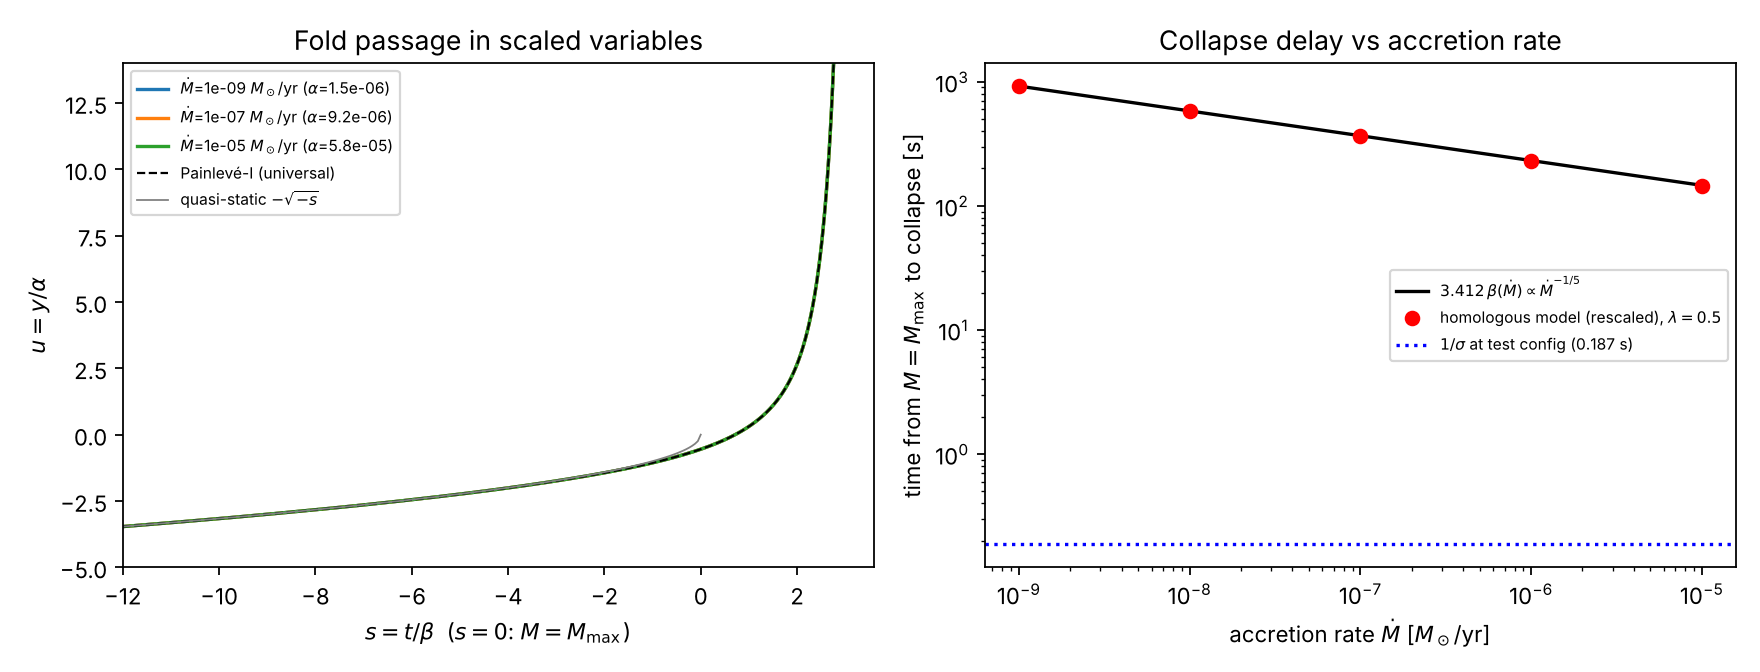
\includegraphics[width=\textwidth]{fig_fold_passage.png}
\caption{Left: fold passage in scaled variables for three accretion rates, which collapse onto the universal Painlevé-I curve (dashed). Right: delay from $M_{\max}$ to collapse against accretion rate, with the $\dot M^{-1/5}$ law.}
\label{fig:fold}
\end{figure}

\paragraph{What this changes.} First, critical slowing-down dominates: collapse follows the crossing of $M_{\max}$ by minutes, not by the $1.2$--$3.8$~s of the seeded runs, because $\sigma\to0$ at the fold; the $0.19$~s e-folding time describes only a star already deep on the unstable branch. Second, the delay is a weak function of $\dot M$ ($\propto\dot M^{-1/5}$): four decades in $\dot M$ move it by a factor $6$. Third, the mass overshoot is $\lesssim5\times10^{-11}\,M_\odot$, so $M_{\max}$ is the collapse mass to that accuracy, the mass at collapse onset; the black-hole mass additionally depends on what happens after onset (Section~\ref{sec:lagrangian}). Fourth, the $\ln(1/\delta_0)$ ambiguity of the previous subsections is replaced by $\delta_{\rm eff}\simeq\alpha\sim10^{-6}$--$10^{-4}$.

\paragraph{Limits.} (i) Conservative dynamics: dissipation is treated separately in Section~\ref{sec:fold-dissipation}; the equations of state here have none, and thermal evolution (a finite-$T$ equation of state) is not included. (ii) Fluctuations: kinetic equipartition for the mode gives $\delta\dot\lambda_{\rm rms}=\sqrt{k_BT/I}\approx6\times10^{-29}\ {\rm s^{-1}}$ at $T\sim10^8$~K (model moment of inertia $I=4.2\times10^{41}$~kg\,m$^2$), i.e.\ $\delta\lambda\lesssim10^{-26}$ over a time $\beta$, far below $\alpha$; thermal noise is therefore not the relevant seed, whereas convective or accretion-driven pulsation, bounded by the amplitude caveat above, would be. (iii) (see also Section~\ref{sec:fold-comp}) The ideal-gas equation of state has no $\beta$-decay thresholds; $\rho_{\max}=2.3\times10^{10}$~g\,cm$^{-3}$ lies above the $^{16}$O threshold ($1.94\times10^{10}$) quoted in Section~\ref{sec:composition}, below $^{12}$C ($3.97\times10^{10}$), so the fold of $^{16}$O (and of $^{56}$Fe, Table~\ref{tab:foldcomp}) is counterfactual, whereas $^{4}$He and $^{12}$C are $\beta$-consistent there; real white dwarfs of those compositions would ignite far below this density. (iv) The single homologous degree of freedom is calibrated on the linear eigenvalue only; its fold-coefficient differs from exact GR by $7\%$, which we report, not hide, and which moves $t_{\rm collapse}$ by $3\%$ and the plunge by $4\%$. The $\dot M^{-1/5}$ scaling and $s_*=3.412$ are properties of the normal form and do not depend on that model.

\subsection{Dissipation in the fold passage}
\label{sec:fold-dissipation}

The fold passage above is conservative. We now ask what dissipation can change. Four channels are considered, and the answer is a bound plus an explicit requirement on microphysics we do not compute.

\paragraph{What cannot change.} Dissipation does not move fixed points: the equilibrium sequence, and hence $\rho_{\max}$ and $M_{\max}$, are those of the equilibrium equation of state, provided the matter relaxes to equilibrium in a time short compared with $\beta$ (otherwise the relevant sequence is the one at frozen composition, with a different turning point). Gravitational radiation from a radial mode vanishes in spherical symmetry (Birkhoff), and shear viscosity does not act on a homologous radial motion. Thermal non-adiabaticity is also negligible here: for degenerate electrons the pressure is nearly independent of temperature, so heat exchange between fluid elements does not change $\Gamma_1$ at leading order. At $\rho_{\max}$ the electron kinetic Fermi energy is $11.2$~MeV, so $(k_BT/E_F)^2=6\times10^{-7}$ at $T=10^8$~K, and the ion thermal pressure is $1.5\times10^{-3}$, $4.9\times10^{-4}$, $3.7\times10^{-4}$ and $1.1\times10^{-4}$ of the electron pressure for $^4$He, $^{12}$C, $^{16}$O and $^{56}$Fe. That ion term is a finite-temperature correction to the equation of state itself (we use $T=0$), not a dissipation, and we do not evaluate its effect on $M_{\max}$.

\paragraph{Damped normal form.} Adding a friction $\nu\dot y$ to Eq.~\eqref{eq:fold-nf} and using the scalings above gives $u''+\tilde\nu u'=u^2+s$ with $\tilde\nu=\nu\beta$. For $\tilde\nu\gg1$ the motion is overdamped, $\tilde\nu u'\simeq u^2+s$, and a second rescaling ($\beta'=(4a\nu^2/\kappa^2\dot M)^{1/3}=\beta\tilde\nu^{2/3}$) reduces it to the Riccati equation $w'=w^2+\tau$. Its solution that follows the equilibrium is $w=-\phi'/\phi$ with $\phi=\mathrm{Ai}(-\tau)$, which diverges at the first zero of the Airy function, $\tau_*=-a_1=2.33811$ \citep[][\S9.9]{DLMF}. This is the first-order (overdamped) form of the jump delay at a fold under a slowly varying parameter, the class of problem treated in \citet{Haberman1979}. Hence
\begin{equation}
t_{\rm collapse}\to 2.338\,\beta\,\tilde\nu^{2/3}\quad(\tilde\nu\gg1),\qquad t_{\rm collapse}=3.412\,\beta\quad(\tilde\nu=0).
\end{equation}
Numerical integration from the first-order adiabatic start gives the crossover in Table~\ref{tab:damped}; the pole position approaches the Airy law from above (ratio $1.07$ at $\tilde\nu=10$).
\begin{table}[ht]
\centering\footnotesize
\begin{tabular}{rrrr}
\hline
$\tilde\nu=\nu\beta$ & $s_*=t_{\rm collapse}/\beta$ & $2.338\,\tilde\nu^{2/3}$ & ratio\\
\hline
0 & 3.412 & --- & ---\\
0.1 & 3.519 & 0.504 & ---\\
0.3 & 3.732 & 1.048 & ---\\
1 & 4.447 & 2.338 & 1.90\\
3 & 6.307 & 4.863 & 1.30\\
10 & 11.63 & 10.85 & 1.07\\
\hline
\end{tabular}
\caption{Collapse delay of the damped normal form $u''+\tilde\nu u'=u^2+s$ (units of $\beta$) against the overdamped Airy law.}
\label{tab:damped}
\end{table}
Dissipation therefore only delays collapse, and does so slowly: the delay grows as $\nu^{2/3}$. The mass accreted before collapse is $\Delta M=\dot M t_{\rm collapse}=2.338\,\dot M^{2/3}(4a/\kappa^2)^{1/3}\nu^{2/3}$ in the overdamped regime. For $\dot M=10^{-7}\,M_\odot$/yr ($\beta=107.7$~s) and $\nu=10\ {\rm s^{-1}}$ (an energy e-folding time of $0.1$~s, $\tilde\nu\approx1100$) this gives $t_{\rm collapse}\approx2.6\times10^4$~s and $\Delta M\approx8\times10^{-11}\,M_\odot$; for $\dot M=10^{-5}\,M_\odot$/yr and $\nu=100\ {\rm s^{-1}}$ it is $8\times10^{-9}\,M_\odot$. The collapse mass is $M_{\max}$ to that accuracy for any damping rate of astrophysical interest.

\paragraph{Bulk viscosity from a relaxing composition, and the requirement it imposes.} The one channel that can act on a radial mode is bulk viscosity from a relaxing internal variable (weak interactions, in dense matter). In the standard relaxation form \citep[][\S81]{LandauLifshitzFM} the real part of the bulk viscosity is $\zeta=\rho\,(c_\infty^2-c_0^2)\,\tau/(1+\omega^2\tau^2)$, with $c_\infty$ and $c_0$ the frozen and equilibrium sound speeds and $\tau$ the relaxation time. For the homologous mode the compression rate $\nabla\!\cdot\!\mathbf v=3\dot\lambda/\lambda$ is uniform, so the energy balance $\dot E=-\int\zeta(\nabla\!\cdot\!\mathbf v)^2dV$ gives $\nu=9\int\zeta\,dV/I$. In the quasi-static limit $\omega\tau\ll1$ appropriate to a ramp with $\omega\sim1/\beta$, and writing $\Delta_r=(c_\infty^2-c_0^2)/c_0^2$,
\begin{equation}
\nu=\frac{9\,\bar\Gamma_1W_P}{I}\,\Delta_r\tau=6.5\times10^{3}\ {\rm s^{-2}}\;\Delta_r\tau,
\end{equation}
using the fold-configuration values $\bar\Gamma_1=1.337$, $W_P=\int P\,dV=2.30\times10^{44}$~J and $I=4.24\times10^{41}$~kg\,m$^2$. Damping matters ($\tilde\nu\gtrsim1$) once $\Delta_r\tau\gtrsim5.7\times10^{-7}$, $1.4\times10^{-6}$ and $3.6\times10^{-6}$~s for $\dot M=10^{-9}$, $10^{-7}$, $10^{-5}\,M_\odot$/yr. This is a small number: a relaxation of relative strength $\Delta_r=10^{-3}$ with $\tau\gtrsim1.4$~ms is enough at $\dot M=10^{-7}\,M_\odot$/yr. It is therefore not safe to assume dissipation is irrelevant for compositions with active weak processes. For the equations of state treated here, which have no relaxing internal variable, $\Delta_r=0$ and the fold passage above is exact within the leading-order normal form. For the $\dagger$ compositions, a value of $\Delta_r\tau$ would require a reaction network (electron-capture and Urca rates near the thresholds), which we do not attempt. What we can say is that collapse occurs at $M_{\max}$ whatever the damping, after a delay that is at least $3.41\beta$, increases monotonically with $\tilde\nu$ as in Table~\ref{tab:damped}, and approaches the Airy law from above for $\tilde\nu\gg1$ (the Airy law is an asymptote, not a bound).

\subsection{A fully inhomogeneous test: spherical general-relativistic Lagrangian evolution}
\label{sec:lagrangian}

The homologous model has one degree of freedom, and its self-gravity is calibrated rather than derived. We therefore test it against an independent evolution that has neither restriction: the spherically symmetric Misner--Sharp equations in comoving (rest-mass) coordinates \citep{MisnerSharp1964,MayWhite1966}, with the same equation of state and the same TOV initial profile.

\paragraph{Scheme.} The unknowns are the radius $r_j$, proper velocity $U_j=dr/d\tau$ and Misner--Sharp mass $m_j$ at the zone interfaces of a grid in rest mass $\mu$ (spacing $\propto(1-x)$ toward the surface). The relations used are $\Gamma^2=1+U^2/c^2-2Gm/rc^2$, $\rho=\bar\Gamma\,\Delta\mu/V$ with $V=\tfrac{4\pi}{3}(r_{j+1}^3-r_j^3)$, $dm=eV/c^2$ across a zone (Hamiltonian constraint), $dm/d\tau=-4\pi r^2PU/c^2$ and
\begin{equation}
\frac{dU}{d\tau}=-\Gamma c^2\,\frac{4\pi r^2\,\Delta P}{h\,M_{\rm node}}-\frac{G}{r^2}\Big(m+\frac{4\pi r^3P}{c^2}\Big),
\end{equation}
which is the Euler equation $-\Gamma^2c^2\,\partial_rP/(e+P)$ with the node inertia written through the node's rest mass $M_{\rm node}$ and enthalpy per unit rest mass $h=(e+P)/\rho$. For a barotropic fluid in comoving slicing $\alpha h$ is spatially constant, so the lapse is fixed by matching the exterior Schwarzschild time at the surface, $\alpha_s=(1-2GM/Rc^2)/\Gamma_s$; times below are this exterior coordinate time (the surface event of each comoving slice), the normalization of the eigenvalue $\sigma$, which the linear tests below fix to about $0.1\%$. We integrate with fourth-order Runge--Kutta at a Courant number $0.4$ (at $N=200$ the times $t(\lambda_h=0.5)$, $t(0.15)$ and $t_{\rm AH}$ at Courant numbers $0.2$, $0.4$ and $1.2$ agree to $4\times10^{-8}$~s; the interpolated $m_{\rm AH}$ changes by $2\%$). There is no artificial viscosity. The residual of the discrete initial equilibrium is subtracted from the force bracket (a well-balancing step, the same device as the $R_0$ subtraction of the homologous model; it is a standard device for well-balanced schemes, but here it is heuristic and justified only by the convergence tests below); at the outermost node this residual is not small ($\approx0.5$ of local gravity), which is a plausible cause of the sub-second-order convergence below, although that node carries under $10^{-4}$ of the mass.

A first version of this scheme took the node inertia from an arithmetic mean of zone enthalpy densities. It was not mass-consistent where the density changes by factors of 2--4 between zones near the surface, and a Jacobian eigenvalue analysis showed a spurious surface-trapped growing mode (that version is not part of the release). The mass-based form above removes it: all eigenvalues of the stable-branch configuration then have real parts of magnitude at most $4\times10^{-10}\ {\rm s^{-1}}$ (round-off; $N=100$ to $800$, \texttt{lag\_eigs.py}). (An earlier, strong-form Lagrangian code on a preliminary configuration developed shell crossing \citep{OwnbyPhase2}; we have not isolated why. Here the minimum zone width stays positive and $\Gamma^2\ge0.41$ in every run.)

\paragraph{Validation against the linear results.} The eigenvalues of the discrete Jacobian provide two tests that do not use the pulsation equation. (i) On the fiducial configuration ($\rho_c=5\times10^{10}$~g\,cm$^{-3}$) the unstable growth rate is $5.013$, $5.237$, $5.309$, $5.333\ {\rm s^{-1}}$ for $N=100$, $200$, $400$, $800$ zones. Successive differences shrink by $3.1$ per doubling, which is convergence of order $\approx1.6$, not second order; extrapolating with the observed ratio from the first three levels predicts $5.3325$ at $N=800$ (found: $5.3326$) and the limit is $5.3435\ {\rm s^{-1}}$ (assuming exactly second order would give $5.340$), against $\sqrt{28.55}=5.343\ {\rm s^{-1}}$ from Rayleigh--Ritz. (ii) At the turning point $\rho_c=\rho_{\max}$ the lowest discrete $\sigma^2$ is $1.585$, $0.521$, $0.170$, $0.055\ {\rm s^{-2}}$ for $N=100$ to $800$, extrapolating to $-0.0004\ {\rm s^{-2}}\approx0$, an independent confirmation of the turning-point theorem. On the stable branch ($\rho_c=10^{10}$~g\,cm$^{-3}$) the fundamental frequency is $2.922$, $2.842$, $2.815$ against $2.802\ {\rm rad\,s^{-1}}$ (Rayleigh--Ritz) for $N=100$, $200$, $400$. These tests share the equation of state, the TOV profile and $\rho_{\max}$ with the rest of the paper, so they check the dynamics and linearization, not the thermodynamics.

\paragraph{Collapse from the fold, compared with the homologous model.} Because the discrete fold lies at $\sigma^2_N=+0.17\ {\rm s^{-2}}$ for $N=400$ (equivalent to $y\approx0.009$), a hand-off at $y=10^{-2}$ lies inside the discretization error and the discrete star bounces. We therefore hand off at $y=0.1$ ($\sigma^2\approx-1.9\ {\rm s^{-2}}$): the state $(\lambda,\dot\lambda)$ of the homologous model at that point, applied as a homologous displacement and velocity of the $\rho_c=\rho_{\max}$ star (with $\dot\lambda$ read as $dr/d\tau$; reading it as $dr/dt$ would shift $t(0.5)$ by $-0.11\%$), is the initial data for both calculations. Table~\ref{tab:lag} compares them.
\begin{table}[ht]
\centering\footnotesize\setlength{\tabcolsep}{4pt}
\begin{tabular}{lrrrrr}
\hline
 & $t(\lambda_h=0.5)$ [s] & $t(0.15)$ [s] & plunge [s] & $t_{\rm AH}$ [s] & $m_{\rm AH}/M$\\
\hline
Lagrangian $N=200$ & 1.9209 & 1.9745 & 0.0536 & 1.9777 & 0.178\\
Lagrangian $N=400$ & 1.7622 & 1.8155 & 0.0533 & 1.8187 & 0.175\\
Lagrangian $N=800$ & 1.7200 & 1.7731 & 0.0532 & 1.7763 & 0.177\\
Lagrangian $N=1600$ & 1.7071 & 1.7602 & 0.0531 & 1.7633 & 0.176\\
Lagrangian, extrapolated & $1.702\pm0.002$ & $1.755\pm0.002$ & 0.053 & $1.758\pm0.002$ & $0.176\pm0.003$\\
Homologous, rescaled & 1.7083 & 1.7601 & 0.0518 & --- & ---\\
Homologous, raw & 1.7595 & 1.8133 & 0.0538 & --- & ---\\
\hline
\end{tabular}
\caption{Collapse from the fold, starting at $y=0.1$ (Lagrangian: half-rest-mass radius ratio $\lambda_h$; $t_{\rm AH}$: first time $\max_r2Gm/rc^2=1$ on the comoving slices; $m_{\rm AH}$ interpolated to that instant, uncertain by about $\pm0.003$ because the maximum shifts between nodes). Times are from the hand-off state; ``rescaled'' uses the exact-GR fold coefficient. The extrapolation uses the observed difference ratios ($3.8$, $3.3$, trending to $\approx3$), and the error is the spread between ratios $3$ and $4$.}
\label{tab:lag}
\end{table}
The Lagrangian time to $\lambda_h=0.5$ converges at order $\approx1.7$--$1.9$ (differences $0.159$, $0.042$, $0.013$~s) to $1.702$~s, $0.4\%$ from the rescaled homologous model ($0.5\%$ with the velocity convention above) and $3.4\%$ from the raw one. The plunge from $\lambda=0.5$ to $0.15$ is $0.0531$~s against $0.0518$ (rescaled, $-2.5\%$) and $0.0538$~s (raw, $+1.3\%$); neither calibration matches both timings better than $1$--$2.5\%$. Two caveats on how much this agreement shows. First, the initial data, the equation of state and the fold coefficient are shared, and about $85\%$ of $t(0.5)$ is spent at $\lambda>0.8$, in the weakly nonlinear regime governed by $\kappa$ and $a$, so the $0.4\%$ mainly confirms that the Lagrangian and Rayleigh--Ritz fold coefficients agree to about $1\%$. Second, the genuinely nonlinear test is the plunge, and there the one-mode model is good to a few percent (the choice of shell, up to $90\%$ of the mass, changes the Lagrangian plunge by only $0.0522$--$0.0541$~s). This is a test of the homologous ansatz against the inhomogeneous dynamics for these initial data, with the homologous model's own state as the starting point; it is not a test of how the star would arrive there.

\paragraph{Through the model's wall, to a first trapped shell.} The Lagrangian code is not limited by the model's frozen-metric breakdown at $\lambda\approx0.15$. It continues until $\max_r2Gm/rc^2$ reaches $1$ (a first trapped shell on comoving slices, not an invariant statement about the event horizon), which occurs $0.0563$~s after $\lambda_h=0.5$ ($0.0568$, $0.0565$, $0.0563$, $0.0563$~s for $N=200$ to $1600$), only $0.003$~s after $\lambda_h=0.15$. It first appears at an interior shell enclosing $m_{\rm AH}=(0.176\pm0.003)\,M=0.249\pm0.004\,M_\odot$, and at that moment the central rest-mass density has risen by a factor $\approx3\times10^{7}$ ($2.5$, $2.9$, $3.1$, $3.2\times10^{7}$ for $N=200$ to $1600$, a zone average, not converged). The collapse is strongly inhomogeneous at the end, so the homologous ansatz has long ceased to describe the shape: relative to their initial radii the shells enclosing $5\%$, $20\%$, $50\%$, $80\%$, $95\%$ and $99\%$ of the rest mass sit at about $0.0036$, $0.0054$, $0.0127$, $0.030$, $0.060$ and $0.091$ ($N=1600$), and the surface at $0.167$--$0.174$ ($N=200$ to $1600$). What the model gets right is the timing up to the point where it is still valid, which is set by the core. The Hamiltonian-constraint violation stays $\lesssim8\times10^{-8}$ of $M$ until $\lambda_h\approx0.2$ ($8.0\times10^{-8}$, $2.7\times10^{-8}$, $8.8\times10^{-9}$, $3.9\times10^{-9}$ for $N=200$ to $1600$) and rises at the first trapped shell to $2.6\times10^{-5}$, $5.7\times10^{-6}$, $1.2\times10^{-6}$, $2.4\times10^{-7}$. Script: \texttt{fold\_trapped\_diag.py}.

\paragraph{Limits.} (i) The equation of state is the ideal cold electron gas throughout. At $\lambda_h=0.5$ the central density is already above the $\beta$-capture thresholds, and by the first trapped shell it is $\sim6$--$7\times10^{17}$~g\,cm$^{-3}$, beyond nuclear density, with $P/\rho c^2\approx0.46$ in a gas whose baryons are pressureless. A realistic star would neutronize and could bounce; the trapped shell, the seed mass $0.25\,M_\odot$ and the post-$\lambda=0.5$ timing are properties of this model, not predictions for stars. The agreement with the homologous model, by contrast, is a test of dynamics under the same equation of state, and an equation-of-state error cancels between the two calculations. (ii) Spherical symmetry only: non-radial modes are not included (not treated in this paper). (iii) Only the first trapped shell is reported; accretion of the remaining $\approx1.17\,M_\odot$ onto it was not followed, because exterior time freezes there. (iv) The density floor in the equation-of-state routine (below $10^{-3}$~kg\,m$^{-3}$) is never reached here and would need replacing for an expansion or bounce run.

\subsection{Composition dependence of the fold passage}
\label{sec:fold-comp}

The fold coefficients were measured for each Salpeter-lattice equation of state of Section~\ref{sec:composition} by the same procedure as for the ideal gas ($\rho_{\max}$ by an optimizer with tolerance $10^{-8}$ in $\log\rho$, although the flat mass peak limits its accuracy to $\sim3\times10^{-5}$, which does not affect $\kappa$ and $a$ as symmetric differences; $\kappa$ and $a$ from the symmetric differences at $y=\pm0.005,\pm0.01$, 12000-point solver). Table~\ref{tab:foldcomp} gives them with the consequent collapse delay $s_*\beta=3.412\,\beta$ at $\dot M=10^{-7}\,M_\odot$/yr.
\begin{table}[ht]
\centering\scriptsize
\begin{tabular}{lrrrrrrrr}
\hline
 & $\rho_{\max}$ [g\,cm$^{-3}$] & $M_{\max}$ [$M_\odot$] & $\rho_\beta$ [g\,cm$^{-3}$] & consistent? & $\kappa$ [s$^{-2}$] & $a$ [$10^{-3}M_\odot$] & $\beta$ [s] & $t_{\rm coll}$ [s]\\
\hline
ideal ($\mu_e=2$) & $2.311\times10^{10}$ & 1.4166 & --- & --- & 18.73 & 4.027 & 107.7 & 367\\
$^{4}$He & $2.346\times10^{10}$ & 1.4013 & $1.39\times10^{11}$ & yes & 18.99 & 3.976 & 106.8 & 365\\
$^{12}$C & $2.386\times10^{10}$ & 1.3849 & $3.97\times10^{10}$ & yes & 19.26 & 3.922 & 105.9 & 361\\
$^{16}$O$^\dagger$ & $2.402\times10^{10}$ & 1.3782 & $1.94\times10^{10}$ & no & 19.38 & 3.900 & 105.6 & 360\\
$^{56}$Fe$^\dagger$ & $2.932\times10^{10}$ & 1.1507 & $1.18\times10^{9}$ & no & 22.44 & 3.094 & 95.0 & 324\\
\hline
\end{tabular}
\caption{Fold coefficients and collapse delay at $\dot M=10^{-7}\,M_\odot$/yr for the lattice-corrected equations of state. $\rho_\beta$ is the $\beta$-decay threshold of \citet[Table~II]{RotondoRRX2011}; ``consistent'' means $\rho_{\max}<\rho_\beta$. The $\dagger$ rows lie above their threshold, so matter of that composition would have neutronized before reaching the fold. $t_{\rm coll}=s_*\beta$ is the time to the normal-form pole; Table~\ref{tab:fold} gives the time to $\lambda=0.5$ in the full model (366~s against 367~s here at the same $\dot M$).}
\label{tab:foldcomp}
\end{table}
Two points follow. First, the fold passage is nearly composition-independent: $\kappa$ rises by $1$--$20\%$ and $a$ falls by $1$--$23\%$, and the delay changes by $1$--$2\%$ ($^{4}$He, $^{12}$C, $^{16}$O) to $12\%$ ($^{56}$Fe), because $t\propto(a/\kappa^2)^{1/5}$ is a weak function of both. The seed $\alpha\propto\kappa^{-1}\beta^{-2}$ changes by at most about $7\%$. Second, unlike the fiducial density $5\times10^{10}$~g\,cm$^{-3}$ of the seeded runs, which exceeds the $^{12}$C threshold, the fold itself lies below the $^{12}$C and $^{4}$He thresholds, so for these two compositions the equation of state is self-consistent at the fold and there is no relaxing weak process there ($\Delta_r=0$ in Section~\ref{sec:fold-dissipation}). This does not make the scenario realistic: nuclear burning (carbon and helium ignition, pycnonuclear fusion) is not in the model and acts at far lower densities in real stars, so these rows describe a counterfactual non-burning star whose only role is to show that the fold analysis does not depend on the choice of lattice composition.

\subsection{What this does, and does not, establish}
\label{sec:timescale-honest}

This calculation is a genuine nonlinear result, not merely the linear eigenvalue restated: it evolves the fully nonlinear internal energy (exact, via the barotropic identity, with no $\Gamma_1$-linearization anywhere) and the fully nonlinear self-gravity of the frozen background, with a relativistic correction calibrated against the linear eigenvalue, through the entire trajectory, including deep into the regime where the perturbation is far from infinitesimal, and it reproduces, independently, the qualitative two-phase structure (slow exponential onset, fast dynamical plunge) that the physics should produce. It is not a replacement for a genuine nonlinear, inhomogeneous, strong-field numerical-relativity evolution: it is restricted by construction to one homologous degree of freedom (Chandrasekhar's own linear calculation shows this is already an excellent, $13\%$, approximation to the true unstable eigenfunction; a two-mode extension, Section~\ref{sec:twomode}, changes the growth phase by $1.2$--$1.5\%$ and the plunge time by $\approx9\%$), which need not remain an equally good approximation once the collapse is highly nonlinear and the frozen-metric treatment of self-gravity is calibrated, not derived, for exactly the regime where it is least trustworthy. We regard the $e$-folding time $1/\sigma\approx0.19$~s as a direct, essentially assumption-free consequence of the already-validated linear eigenvalue (any model built to reproduce $\sigma^2=-27.85$ in its linear limit gives this number), the dynamical-plunge time $\tau_{\rm plunge}\approx0.03$~s as a physically reasonable, order-of-magnitude estimate consistent with the star's own dynamical time, and the total few-second collapse timescale of the seeded runs as the honest combination of the two, explicitly flagged as dependent on an astrophysically undetermined initial perturbation size (for a star reaching $M_{\max}$ by slow accretion this is superseded by Section~\ref{sec:fold}: minutes, with the seed set by the accretion rate). A fully nonlinear, inhomogeneous, strong-field evolution --- identified in Section~\ref{sec:nonlinear-outcome} and costed in the supplementary technical report \citep{OwnbyPhase2} --- is needed to check whether the homologous ansatz survives into the deeply nonlinear regime and to follow the collapse through the compactness threshold at which this model stops. Section~\ref{sec:lagrangian} supplies a spherically symmetric version: it confirms the homologous timing to $0.3$--$0.5\%$ in the time to $\lambda=0.5$ (though that agreement mostly tests the linear fold coefficient) and to a few percent in the plunge (the genuine nonlinear test), and follows the collapse to a first trapped shell, all within the idealized equation of state; non-radial modes and a realistic high-density equation of state remain.

\section{Discussion}
\label{sec:discussion}

\subsection{What is established}

For the idealized cold electron gas in general relativity: the maximum mass is $1.4166\,M_\odot$, within $0.07\%$ of Chandrasekhar and Tooper; Chandrasekhar's pulsation equation, with the term our first implementation omitted and the energy density used consistently, gives a fundamental eigenvalue that vanishes at the mass maximum to within $0.007\%$ in central density for five equations of state, so the instability sets in where the turning-point principle says it must \citep{HTWW1965,HadzicLin2021}. At the test configuration $\sigma^2=-28.55\ {\rm s}^{-2}$ ($e$-folding $0.187$~s). Here $\sigma^2<0$ is a linear instability; we interpret it, following Friedman's criterion \citep{FriedmanLectures}, as carrying negative canonical energy (we did not compute $E$ for the relativistic mode), and the numerical-relativity literature \citep{FontEtAl2002,RadiceRezzollaKellermann2010} exhibits the nonlinear fork on polytropic stars (collapse for compressive perturbations, migration to the stable branch for expansive ones); the fork is taken from the literature, not from our own code, and is assumed to carry over to the degenerate gas.

What is ours is quantitative. The calibrated homologous model, compared with the independent Lagrangian evolution ($0.4\%$ in the time to half the radius, $1$--$3\%$ in the plunge), gives the exponential-then-plunge trajectory. For accretion the passage through the fold is a ramped saddle-node described by Painlev\'e~I, with $t=3.41167\,(4a/\kappa^2\dot M)^{1/5}$, a delay $\propto\dot M^{-1/5}$, an overshoot below $10^{-10}\,M_\odot$ in the conservative case, a composition dependence of $1$--$12\%$, and a dissipation that can only lengthen the delay. The Painlev\'e~I scaling at a saddle-node of a self-gravitating fluid is known in the Newtonian setting \citep{Pomeau2014,Chavanis2020}, where it governs the early collapse of a supernova core as a control parameter (temperature, respectively energy) is slowly ramped through a saddle-node (saddle-center) of the equilibrium sequence; the relativistic fold coefficients are what we add.

\subsection{What is not established}

(i)~The matter is an idealized gas that does not neutronize; Paper~D \citep{PaperD} replaces it with dense-matter equations of state and finds that the real core bounces at $1.3$--$3.5\,\rho_{\rm nuc}$, so the trapped shell of $0.25\,M_\odot$ found here is a property of the toy gas and not a prediction. (ii)~The one-mode model is calibrated, not derived; its agreement with the Lagrangian evolution is a consistency check at the stated tolerance, not a proof. Its heuristic elements are the single calibration factor $f_{\rm cal}$ (fixed by one linear eigenvalue), the use of the frozen equilibrium background in the force, the subtraction of the equilibrium residual $R_0$, the empirical offset $c\approx0.63$ in the growth-phase formula (a fit, not derived), and the rescaling of the force to the exact-GR fold coefficient; the Lagrangian scheme has a corresponding well-balancing subtraction (Section~\ref{sec:lagrangian}). None is validated by a derivation, only by the cross-checks reported. (iii)~Our Lagrangian scheme fails the relativistic Noh test (documented in Paper~D \citep{PaperD}), so the plunge duration is not claimed beyond the $1$--$3\%$ agreement of Section~\ref{sec:lagrangian}, and Paper~D finds that the plunge duration depends on where the evolution is handed off. (iv)~Our earlier from-scratch nonlinear attempts failed to converge on an outcome \citep{OwnbyPhase2}; they are not used here and no claim rests on them. (v)~Nothing in this paper bears on the quantum or regularized interior: it concerns only whether collapse of this matter proceeds to the regime in which the question arises.

\subsection{Relation to the rest of the series}

Nothing here revises Papers A or B. Paper~D \citep{PaperD} carries the analysis to a realistic equation of state, where the remnant is a neutron star of $1.29$--$1.36\,M_\odot$ unless a second fold is crossed, and Paper~E \citep{PaperE} turns to what happens inside a black hole of the mass-dependent family once it forms.

\section*{Code and data availability}

All numerical results and figures of this paper are produced by the Python scripts in the Paper~C repository, archived on Zenodo at \href{https://doi.org/10.5281/zenodo.23455581}{doi:10.5281/zenodo.23455581} (the repository also contains this manuscript's \LaTeX\ source). Running \texttt{bash verify.sh} in the archive runs all scripts, compares 872 quoted numbers and statements with the computed ones and writes \texttt{verification/REPORT.md} (quick tier about 22 CPU-minutes; \texttt{--full} adds about 162 CPU-minutes, of which about 25 for the Lagrangian re-do of the technical report); every statement marked verified symbolically is backed by a SymPy/mpmath script in \texttt{code/symbolic/} with its log. Its \texttt{README.md} lists, for every table, figure and quoted number, the script that produces it, the output file and the run time; the scripts use relative paths and the shipped logs and \texttt{.npy} files are the outputs on which the tables are based. The code needs Python~3 with NumPy ($\geq2.0$), SciPy and Matplotlib (the tested versions are listed in \texttt{requirements.txt}); most scripts run in seconds to a few minutes and the longest (the composition survey) in about fifteen minutes on a shared two-core machine. No external data are used: the equations of state are analytic (Chandrasekhar degeneracy with a Salpeter lattice correction), and all constants are defined in the code. The supplementary technical report \citep{OwnbyPhase2} and the Newtonian solver scripts used in Section~\ref{sec:galerkin-main} are in the subdirectory \texttt{technical\_report\_phase2}; some scripts of that report were not retained, as stated in its README. The file \texttt{PROVENANCE.md} in the repository root lists every file that differs from the original archive (Zenodo version 1.0.1) and why, the scripts and figures that are re-creations without an original (\texttt{fig1\_pekeris.py}, \texttt{fig8\_collapse\_timescale.py}, \texttt{figs\_friedman.py} and the figures they write; the originals of these three figures are kept in \texttt{figures\_original/}), the shipped logs that are superseded (\texttt{code/survey3.log}, \texttt{code/survey3.json}), and the results that changed relative to the original archive.

\bibliographystyle{plainnat}
\bibliography{references}

\end{document}
